\part{Semantic Representation}
\label{part:semantic-representation}

\chapter*{Abstract}
\label{chap:semantic-representation_abstract}
- Terrain generation usually focus on geometry processing \\
- Some works include soil materials in their process \\
- But no semantic information is preserved \\
- Many fields use topologic maps to describe the environment \\
** see Travel books \\
- Our method to abstract the geometry and focus on the symbolic \\
- ... 


% Automated terrain generation is a key component of natural scene digital modeling for animated movies and video games. Many landscapes have been studied and are synthesised with more and more realism. 
% Different processes can be used and combined to achieve these scenes: fractal terrains \cite{Musgrave1989,Prusinkiewicz1993a}, erosion simulation \cite{Cordonnier2023, Mei2007}, manual modeling \cite{DeCarpentier, Guerin2022}, geological simulation \cite{Cortial2019,Cordonnier2017a}, ... The high quality of synthesis for such environment is due to the possibility to observe these environments from many point of views: long-distance gazing, hiking on mountains, remote sensing, aerial imaging, ... 
% Thanks to the quality of the digital modeling, the entertainment industry display often breathtaking land scenes.

% Underwater scenes are rarely created in these media for multiple reasons: these environments are not completely understood and mastered as much as land environments because they are difficult to access, we lack the capacity to see them at a larger scale (unlike mountains for example) and the underlying process that forms these landscapes are much more complex to simulate.

% These limitations cause animated movies and video games studios to avoid as much as possible underwater environments. 

% However, these environments are important for the study of biology, geology, and, by extension, robotics. Due to the complexity, limitations and danger of underwater human operations, underwater robots are more and more used for marine environment monitoring\cite{Maslin2021, Williams2016, Dunbabin2020, Palmer2021}. Yet the validation process of such underwater robot is expensive, with heavy logistic, and it is often  impossible to find the appropriated environment to test the system. Thus, underwater robotics requires simulation capacities, to be able to test the robot's algorithms in very specific environment and conditions. But for now, roboticians are lacking the capacity to test on realistic virtual scenes, and so only test them on synthetic scenarios that do not correlate with real world terrains. For that, they need to manipulate more precisely the characteristics of the underwater environment, at different scales.

% The difficulties to visualize and study the underwater environments on a large scale at the same time as a small scale is an obstacle to the procedural generation and simulation of scenes that are coherent in these two different scales. 
% A solution to this problem could be a bottom-up approach, simulating at the smallest scale the behaviour of all the elements of the environment. Computing such a simulation in order to generate an entire ecosystem is an near-impossible task due to time and memory complexity. 

% The method we propose provides a way to procedurally generate environments on multiple scales without introducing such complexity by using a sparse representation of the environment using \glosses{EnvObj}.
% The \glosses{EnvObj} only have access to local values of the environments to spawn, grow and die. The use of local interaction with environment values removes the need for complex interconnections between all elements of the terrain, providing a parallelisable generation process at large to small scales.
% Defining \glosses{EnvObj} of the terrain as parametric models based on point, curve or region skeletons provides a lightweight representation of the terrain that the user can interact with. The interaction with the simulation process is still a difficult task \cite{Smelik2014}.
% Our method does not aim for a visually realistic generation, but for a plausible terrain depending on geological and biological constraints, guided by the user. Using state of the art modeling of the geometry of the \glosses{EnvObj} of the terrain could achieve realistic results. We illustrate the method through the generation of coral islands and reefs.

% Our main contribution are the introduction of a sparse representation of the terrain elements as \glosses{EnvObj}, the use of fitting functions to incorporate biological rules in the simulation process avoiding physic simulation and an interactive simulation based on geological \glosses{GeoEvent} for underwater landscapes.




% Simulating underwater landscape growth is complex due to the interplay of biological, environmental, physical, geological, and human factors. Our method addresses this complexity by introducing a sparse representation of the terrain elements using environmental objects, defined as parametric models based on point, curve, or region skeletons, which interact locally to spawn, grow, and die. This approach removes the need for complex interconnections, enabling a parallelizable and scalable generation process. By using fitting functions to incorporate biological rules and focusing on geological plausibility, our method enables interactive underwater landscape simulations. The main contributions of this work are the introduction of sparse terrain element representation, the use of fitting functions to simulate biological processes without complex physics, and the development of an interactive simulation framework based on geological events.

\graphicspath{ {./Chapter 1/} }

\chapter{Generation de terrain sémantique}
\label{chap:semantic-representation}
\minitoc
\teaser{
	 \includegraphics[width=0.9\linewidth]{Figures/Render/figureTeaser.png}
	%  % \centering
	  \caption{Our method can produce different scenes including coral islands and canyons at multi-scale using Semantic Terrain Entities to represent terrain features.}
	\label{fig:semantic-representation_teaser}
	}

% topography
% Representing an environment as a topographic map
% A method that uses new objects, EnvObjs, to represent the landmarks of a terrain
% Our method represents the different landmarks of a terrain using a geometric (as "without 3D repr") representation. To avoid cycles in the interactions between objects, we use the environment as a proxy. EnvObjs are independant, like cellular automata. Each object affects locally the environment by modifying EnvVals. This modifications are applied by the EnvObjs spreading EnvMat around them. They also absorb EnvMat from the other EnvObjs. We can consider that the diffusion is bounded thanks to a decay rate, meaning the system becomes stable after some time. Because it is stable, it is plausible. We break the stability by adding new EnvObjs following \glosses{GenRule}. New EnvObjs are placed in the environment where they may be the most probable, following a fitness function using the EnvVals. Then the shape of the skeleton is defined following a skeleton \gloss{FitnessFunc}. We wait for the environment to stabilize. It can take some time, and some EnvObjs might die (if fitness function fall below 0), but it will converge. The user can guide this process by defining EnvObjs that can spawn. Also, because it is simple skeleton, he can modifie shapes. The diffusion process is deterministic so no abrupt changes in the landscape. Also, the stability of the system can be broken by influencing EnvVals. So user can affect them through \Glosses{GeoEvent}. \Glosses{GeoEvent} affect one or more EnvVal over time, but we reduce the number of evaluation to the begining and end of the \glosses{GeoEvent}. Each EnvObj has a probability of chance to spawn each day, which can be computed as an amount per month, years, etc... (Probability Distribution Function of $p(X) = p^t$).  

\section{Introduction}
% Slight introduction
Topographic maps are very useful tools for biologists, geologists or even oceanologists (which would call them "bathymetric charts"). These maps are displayed in 2D but provide 3D information about the altitude (or depth), but can also use symbology to represent the important elements that need to be visible. Map symbols are important in order to extract as much information as possible from a 2D object. In cartography, map symbols are defined as geometric primitives such as points, polylines, polygons, and (rarely) polyhedrons. These symbols are a simplification of the content of an environment, or an abstraction of the 3D shape of the terrain features. This is useful to understand the relationship between the different features, which enables to deduce rules in the evolution of a terrain. 

% WHo would want it, and why?
In such way, geologists can study the distribution of peaks in a mountain range, the location of soil types in an area, which in turn allow to deduce possible locations of karst networks, for example. Using the same tools, a biologist may interpret the effect of natural or artificaial reefs on coastal erosion, or understand better the interactions inside an ecosystem. Oceanologists may deduce the formation of canyons and fans from old river systems.

The abstraction of the details on the surface allows to focus on the undepth understanding of a process, which may be generalized to different terrain configurations. 

Parallelly, terrain artists most of the time sketch the global shape of the terrain they will model beforehand, such that they can check before the modeling part that the consistency and plausibility of the terrain will be valid. Looking at a simplified map before starting the modeling step allows the designer to modify the overall shape of the terrain, at a large scale, before the 3D geometry comes in play, generating too much control points or vertices to be able to deal with.

Starting from an initial configuration or providing conditions on the desired output terrain, the algorithm we propose will let the different terrain features evolve as a multi-agent system, allowing for a simulation of evolution on multiple years, while, at any time, the user can apply modifications or new constraints on the state of the environment. The resulting configuration is an environment conform to the constraints shared by the user, which can be about the number of years of simulation and/or the distribution of features present in the scene.

% Why it does not already exists?
As described in the previous chapter, most terrain generation algorithm use the geometry of an initial terrain surface to iteratively apply changes such as erosion simulation. While information about some environment variables or properties of the ground may influence the result of an algorithm, the control of the global shape of the terrain is lost as it treat locally the surface, without knowing which feature a certain point on the surface lies on.

% Personal motivation
The question which led to our solution is the multi-scale user interaction: "Is it possible to provide an interaction mean for terrain generation allowing the user to interact with a small structure like a rock in the same manner as with a large structure like a mountain?". 
In this work, we want the user to be able to have a large scale representation of the terrain in order to generate a landscape that satisfies his needs while keeping the possibility to apply large modifications.
In discussion with robotician users, we realise that we want to create a large landscape that can contain interesting , select a smaller region that have features in a disposition that.
In the optic of generating a large scale terrain in which we could focus the generation effort in a certain region, we wished to be able to see a coarse representation that can be computed quickly.

We want this method to be adapted for terrains above and under the water level.

Because many geographical terms would become ambiguous in computer science terms, in which this thesis lie in, we will translate some vocabulary in a way that may be disapproved by geologists, but we are doing our best to keep it as acceptable for each field as possible.


% \subsection{Nomenclature}
% % Geographical feature/entity -> Semantic Terrain Entity
% A geographical feature, also known as a feature, object, or entity, is a discrete phenomenon located at or near the Earth's surface, relevant in geography and geographic information science. It represents geographic information that can be depicted in maps, geographic information systems (GIS), and other forms of geographic discourse. The term "feature" includes both natural and human-made objects, ranging from tangible items like buildings to intangible concepts like neighborhoods. Features are distinct entities with defined boundaries, differentiating them from continuous geographic masses or processes occurring over time. They can be categorized as natural features, such as ecosystems, biomes, water bodies, and landforms, or artificial features, such as settlements, administrative regions, and engineered constructs. Geographic features are described by characteristics including identity, existence, classification, relationships with other features, location, attributes, and temporal aspects. Information about these features is stored in geographic databases using models like GIS datasets, which organize and represent these features in structured formats.
% % A geographical feature, also referred to as a feature, object, or entity, is a discrete phenomenon located at or near the Earth's surface, relevant in geography and geographic information science. It is an item of geographic information that can be represented in maps, geographic information systems (GIS), remote sensing imagery, statistics, and other forms of geographic discourse. The term "feature" is broad and inclusive, encompassing both natural and human-made objects. It includes tangible items like buildings as well as intangible concepts like neighborhoods. Features are discrete entities with distinct identities and locations, characterized by defined boundaries that differentiate them from other objects, distinguishing them from geographic processes, which occur over time, and geographic masses or fields, which are continuous. In geographic information science, "feature," "object," and "entity" are often used interchangeably, although some formal distinctions exist, such as seeing a feature as an abstraction of a real-world phenomenon. Geographical features can be categorized into natural and artificial types. Natural features include ecosystems, which are communities of organisms interacting with their environments; biomes, which are large areas with ecologically similar communities defined by plant structures, climate, and ecological patterns; water bodies, which are significant accumulations of water like oceans and lakes, either distinct or conceptual in nature; and landforms, which are physical structures such as mountains and valleys defined by surface form, location, and topography. Artificial features encompass settlements, which are human communities ranging from small villages to large cities, including infrastructure like roads and buildings; administrative regions, which are social constructs like states and neighborhoods used for organizational purposes; engineered constructs, which are man-made structures such as highways and airports; and cartographic features, which are abstract map representations, such as grid lines and boundaries, that do not physically exist. Geographic features are represented by descriptors of their characteristics, including identity, existence, kind, relationships, location, attributes, and time. Each feature is unique, often identified by names or codes, and its existence refers to its presence in the real world, including features that are proposed or planned. The kind refers to its classification, such as a building or river, while relationships describe spatial, meronomic (part-whole), and genealogical (parent-child) connections with other features. The location provides a description of where a feature is, including its shape and extent, and attributes describe other characteristics, such as population or size, often expressed as text or numbers. Time relates to the temporal aspects of a feature's characteristics, describing changes over time. Information about features is stored in geographic databases, often using vector data models, including GIS datasets, which help represent these features and their various descriptors in a structured format.

% % Field -> Environmental Attribute
% In geography, the term "field" refers to a continuous spatial phenomenon defined across a region, where each point in that region has a specific value of some variable. Unlike discrete objects, which have distinct boundaries and identities, fields represent variations of phenomena occurring over a continuous space, such as temperature, elevation, or precipitation. Fields can be either scalar or vector quantities: scalar fields represent a single value at every point, like temperature, humidity, or elevation, while vector fields represent quantities with both magnitude and direction, such as wind velocity or ocean currents. Examples of fields in geography include topographic fields, where elevation values are distributed across a landscape; climatic fields, where temperature or precipitation values are mapped over a geographic area; and magnetic fields, which capture the intensity and direction of magnetic forces at various points on the Earth's surface. Fields are often represented mathematically using functions or equations that define how the field's value varies over space, including interpolation or modeling techniques to estimate field values at unsampled locations. In Geographic Information Systems (GIS), fields are typically represented as raster data, where a grid of cells captures the continuous variation of a field across a landscape, with each cell holding a value representing the field's magnitude at that location. Fields are crucial for spatial analysis and modeling, allowing geographers to study patterns and processes that vary continuously across space, such as climate change, land surface modeling, and resource distribution. Thus, in geography, a field is a method of representing continuous spatial phenomena, enabling the analysis of patterns and trends across geographic spaces.

% % Event -> Geological Event
% In philosophy, an "event" is defined as an occurrence or happening that takes place at a specific time and location, characterized by its temporal nature and involvement in change or transition. Unlike static objects, events are dynamic and are often considered fundamental constituents of reality. They typically involve transformations from one state to another, such as a tree falling, and are central to discussions about causality, as they can serve as causes or effects within causal chains. Philosophers debate whether events are basic entities or reducible to other kinds of entities, like properties of objects or states of affairs. They also explore how events are individuated and identified, what distinguishes one event from another, and how events relate to objects. Linguistic and logical analyses focus on how events are described in language, often through verbs and predicates, and how they relate to entities involved. Various philosophical theories, such as process philosophy, emphasize events over static entities, offering different frameworks for understanding the nature of events and their role in the structure of reality. Overall, events are crucial for understanding change, causality, and our perception of the world.

% % Visualization

% \subsection{Features on field experts maps}
% - ... 
% \subsection{Topographic/Planimetric maps}
% - ... 

% \subsection{Analogy}
% - Compare our nomenclature with introduction \\
% - ... 

\section{Related works}
\label{sec:semantic-representation_related-works}
Procedural terrain generation has been heavily studied for the last 40 years \cite{Galin2019}. Researches in this topic try to find new solutions to compromise between realism, user control and efficiency \cite{Gain2009}. Using fractal noise parametrized to resemble real landscape has been an important first step \cite{Musgrave1989} as it's a fast and light solution to generate procedurally the appearance of mountains. The lack of user control pushed newer works toward the use of controlled noise by including real DEM in the process through learning \cite{Kapp2020, Brosz2007}, while the rise of deep learning technologies gave higher control to the user through sketches \cite{Guerin2017, Talgorn2018}.

By including expert knowledge of tectonic process and subsurface geology, some algorithms tend to get more realistic \cite{Patel2021, Cortial2019, Michel2016}. 

While these algorithms are able to generate large-scale landscapes, the finer details of the terrain is often computed by the use of erosion simulation \cite{Cordonnier2023, Schott2023, Paris2019}. This process can be expensive in time but results in more plausible surfaces.

All the algorithms aim to reproduce plausible relief in terrestrial landscapes, mostly limited to alpine landscapes, but a lack of research can be found in almost all other biomes. Underwater landscapes generation, for example, has been almost completely absent from literature for many reasons: the difficulty of accessing the area, the lack of visibility under water and the complex physics of underwater geology and biology make the algorithms adapted for this environment scarce. 

The majority of the ocean floor can be represented as a fractal terrain \cite{Mareschal1989}. While stochastic noise can be sufficient to model the ocean floor, this process won't cover areas with the biggest biomass, near shallower waters such as near coasts and islands.

Due to the impossibility to observe the large-scale and the small-scale of underwater environments, some works related to geology model large structures like the profile shape of the coral reef \cite{Bosscher1992}, simulate its surface growth \cite{Li2021}, or use procedural algorithms for single polyp \cite{Abela2015}. We however don't have a mix of the different scales, and neither methods take into account the environment such as the topography or the interaction of different terrain features. This is mainly due to the fact that the evolution time for each scale varies from a span of weeks to thousands of years.

In an ecosystem, any element of the system has an impact on their surrounding. Simulating each physical properties such as shading, heat, humidity may require enormous computation power. By considering these properties as scalar fields surrounding the whole scene, and that features of the terrain affect locally the scalar fields, we can simplify the computation of the physical properties of the environment \cite{Grosbellet2016, Guerin2016a}. This process provides a scalable system from which scene details are rendered in a plausible way. In a similar way, other works represent the wind flow as a composition of local vector fields \cite{Wejchert1991}, avoiding complex fluid simulation while providing user control in a lightweight model. We extend these works by incorporating a time-evolution system such that the scene can be dynamic.


\section{Overview}
\label{sec:semantic-representation_pipeline}

\begin{figure*}
    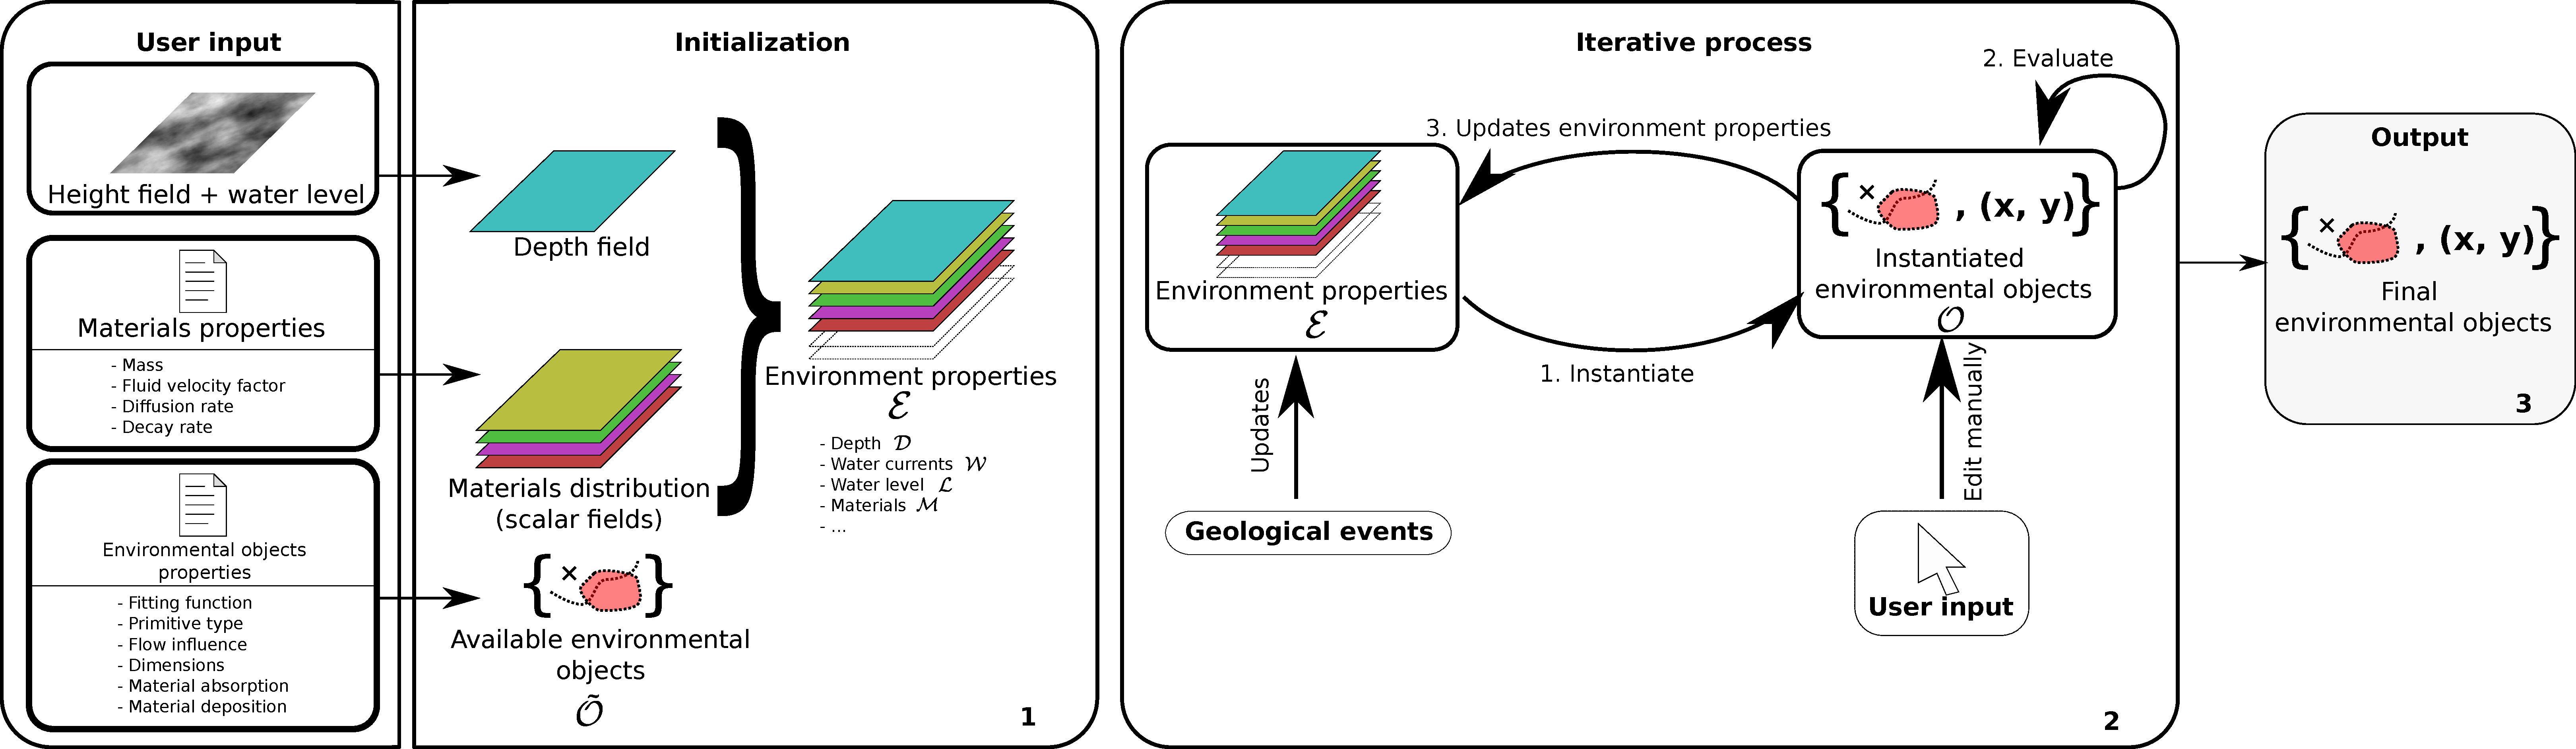
\includegraphics{Figures/pipeline.pdf}
    \caption{Overview of the pipeline of the method. The user provides as input an initial height field and sets the water level, as well as a definition of the \glosses{EnvMat} properties and \glosses{EnvObj} properties that will be used in the iterative process. These inputs are initialized as an initial set of \glosses{EnvObj} and scalar fields that represents the \glosses{EnvVal}. In the iterative loop, new \glosses{EnvObj} are instantiated using the current state of the environment at their optimal position. The existing \glosses{EnvObj} in the terrain reevaluate their \gloss{FitnessFunc} to grow or die and update the \glosses{EnvVal} locally. At each iteration, \glosses{GeoEvent} can update the \glosses{EnvVal}, while the user can interact directly with the \glosses{EnvObj}. The result of the whole process is a set of \glosses{EnvObj} which is a sparse representation of the features of the scene. }
    \label{fig:semantic-representation_pipeline}
\end{figure*}

The generation of the terrain is initialized using an initial height field $\height$ and a water level $\Wlevel$. The height field provides variation on the depth $\depth$, which can influence the generation process of the scene. We set $\depth = \height - \Wlevel$.

The list of available \glosses{EnvObj} $\availableObjects$, representing the different features that can be present in the scene, are provided with their properties: type, size, \glosses{GenRule}, growing conditions and effects on the \glosses{EnvVal} (Section~\ref{sec:semantic-representation_environmental-objects}).

Finally, different \glosses{EnvMat} can be defined with their properties such as diffusion speed, mass, damping factor and influence from the water currents. \Glosses{EnvMat} distributions are represented as a scalar field $\material: \R^2 \to \R$ and water currents as a vector field $\Water: \R^2 \to \R^2$ that can be evaluated by the \glosses{EnvObj} of the scene to simulate their growth and spawn at the most probable position. The environmental properties $\environment = (\depth, \Water, \Wlevel, \material)$ is composed of depth, water currents, water level and \glosses{EnvMat} distribution information at any point of the terrain (Section~\ref{sec:semantic-representation_communication}).

The definition of \glosses{EnvObj}' properties and environment properties is done with field experts, providing the pertinent parameters required to model the evolution of the terrain features using expert knowledge (Section~\ref{sec:semantic-representation_biology}). Additional properties can easily be added to the environment properties $\environment$ in order to fit to the experts needs, such as atmospheric pressure, humidity, temperature, ... 

The generation phase can optionally be started with an initial set of \glosses{EnvObj} present in the scene. 

%- Main loop
Once the initialization phase is done, the generation begins. The generation process is incremental and its main loop is composed of two different steps: the instantiation of new \glosses{EnvObj} then the update of the environment.

% - Object instantiation
At each iteration, new \glosses{EnvObj} can be created at their most fitting locations if possible. The \glosses{GenRule} provided in the initialization phase are used to find the optimal position from stochastic sampling (Section~\ref{sec:semantic-representation_generation-rules}). 
All \glosses{EnvObj} are evaluating their state analytically using the \gloss{FitnessFunc} provided as input (Section~\ref{sec:semantic-representation_obj-evaluation}).

% Once the new objects are instantiated, the process can continue.
% - Environment update
Once the instantiation step is done, the environment's values are updated by each \gloss{EnvObj} by deposing and absorbing some of the available \glosses{EnvMat} (Section~\ref{sec:semantic-representation_materials}) while modifying the water currents (Section~\ref{sec:semantic-representation_water-currents}) around them. Finally, water currents and height field's gradient displace \glosses{EnvMat} of the terrain at each iteration.
% We consider the water currents to be a steady-state flow, allowing us to remove the variation from time in the flow equations.
% The water currents are updated locally by each \gloss{EnvObj} using an analytical form $W^*(\p) = W(\p) + \omega(\p)$.
During the generation process, the user can alter directly the distribution and shapes of the \glosses{EnvObj} (Section~\ref{sec:semantic-representation_manual-interaction}) and perturb the generation process by planning \glosses{GeoEvent} that have impacts on the \glosses{EnvVal} (Section~\ref{sec:semantic-representation_events}).

% - Output result
The output of our system is a set of \glosses{EnvObj} disposed in the plane. We do not provide the 3D representation of the \glosses{EnvObj}, letting the user define the rendering method. The figures used in the paper use a mix of implicit surfaces and triangular meshes.

\subsection{\Glosses{EnvVal}}
\label{sec:semantic-representation_communication}

In geography, a "field" refers to a continuous spatial phenomenon across a region where each point has a specific value of a variable, unlike discrete objects with distinct boundaries. Fields can be scalar, representing a single value at every point (like temperature or elevation), or vector, representing quantities with magnitude and direction (like wind velocity). Examples include topographic fields for elevation, climatic fields for temperature or precipitation, and magnetic fields for magnetic forces. Fields are mathematically modeled using functions and represented in Geographic Information Systems (GIS) as raster data, where a grid of cells captures continuous variations. This representation is essential for studying spatial patterns and processes such as climate change and resource distribution. Because of the ambiguous nature of the term "field" in mathematics and computer science, we will define the geographic fields as \gloss{EnvVal}.

In an ecosystem simulation, each actor of the ecosystem has an impact on all other actors, which results in an exponentially growing computation effort as the number of elements of the terrain increase. We avoid this problem by considering the \glosses{EnvVal} as a proxy to allow any \gloss{EnvObj} to interact with any other one. Each of the \gloss{EnvObj} have a local impact on the \glosses{EnvVal} without knowledge of neighboring \glosses{EnvObj}. This modification of the \glosses{EnvVal} are presented as the effect of \glosses{EnvMat} defined for each \gloss{EnvObj}. % can be due to an absorption and deposition of some material $\material$ or an influence on the water currents.

In this work, we integrated vector \glosses{EnvVal} (water currents $\Water$) and scalar \glosses{EnvVal} (depth $\depth$, water level $\Wlevel$, \glosses{EnvMat} $\material$) into the umbrella "environment" $\environment = \left( \depth, \Water, \Wlevel, \material \right)$. \Glosses{EnvMat} describe a change of \gloss{EnvVal} at one point like an abundance of sand, salt, wetness, rocks, etc... As we do not consider the surface geometry in this work, the reader must restrict himself from seeing it as stacks of materials.


\subsection{\gloss{EnvObj}}
\label{sec:semantic-representation_environmental-objects}
A geographical feature, also called object or entity, is a discrete phenomenon located at or near the Earth's surface, relevant in geography and geographic information science (GIScience). It represents geographic information that can be depicted in maps, geographic information systems (GIS), and other forms of geographic discourse. This term includes both natural and human-made objects, ranging from tangible items like buildings or trees to intangible concepts like neighborhoods or savana. Features are distinct entities with defined boundaries, differentiating them from continuous geographic masses or processes occurring over time. They can be categorized as natural features, such as ecosystems, biomes, water bodies, and landforms, or artificial features, such as settlements, administrative regions, and engineered constructs. Geographic features are described by characteristics including identity, existence, classification, relationships with other features, location, attributes, and temporal aspects. Information about these features is stored in geographic databases using models like GIS datasets, which organize and represent these features in structured formats. As the term "feature" is overused in computer science, we will use the term \gloss{EnvObj} in this work.

Each \gloss{EnvObj} has a simple geometric shape called a "skeleton" that defines where it is located and how it fits into the environment.
These \glosses{EnvObj} interact with the environment $\environment$ by changing local conditions using the \gloss{EnvMat}. For example, a river might increase the moisture in the surrounding area, while a mountain might add rockiness. They can also absorb changes from the environment, such as a forest taking in humidity from the air.
The placement of \gloss{EnvObj} is determined by a \gloss{FitnessFunc}, which evaluates how suitable a location is based on the \glosses{EnvVal}. Once a suitable location is found, the \gloss{FittingFunc} optimizes the shape and position of the entity to fit as best as possible into the environment.


% \Glosses{EnvObj} are rule-based objects following rules depending on their local environment for evaluation their state in their life cycle. We can see them as a life form in the way that they are created and eroded with time. During their lifetime, they influence their local environment by depositing and absorbing \glosses{EnvMat} around them and influencing the water currents. The environment objects are described spatially as a single point, a parametric curve or a region.

\subsection{\Glosses{EnvMat}}
The environment determine if a \gloss{EnvObj} does belong in a position. When a \gloss{EnvObj} is placed, its surrounding \glosses{EnvVal} can be affected though \glosses{EnvMat}. Each \gloss{EnvObj} has intrinsic \glosses{EnvMat} that can be seen as "spreading" and "absorbed" around its skeleton over time. A coral reef may produce coral polyps and at the same time reduce the water currents. It grows thanks to the deposition of [RESIDUS CALCAIRES] from coral colonies. In our model, the colonies affect the \glosses{EnvVal} through the deposition of \gloss{EnvMat} $\material_\text{limestone}$, which in turn, is absorbed by the coral reef, without a direct exchange between the two \glosses{EnvObj}.

The alteration of a scalar \gloss{EnvVal} is done by adding or removing some amount on the skeleton of the \gloss{EnvObj} and diffusing it in the space, influenced by the water currents. We consider the system to be steady-state, garantied by the introduction of a decay rate in the computation of the diffusion.

Altering the vector field of the water currents $\Water$ is done by the addition of the effect of each object at a position $\p$ as introduced in \citep{Wejchert1991}, while we use the formulation of Kelvinlets \cite{DeGoes2017} in the computation of effect of each \gloss{EnvObj}.

\section{Placing \glosses{EnvObj} in an environment}
\label{sec:semantic-representation_generation-rules}
At each iteration of our algorithm, we want our objects to be at plausible positions. We do not guaranty a temporal continuity between iterations as in \citep{Ecormier-Nocca2021}, so the objective is to add new \gloss{EnvObj} in order to satisfy the users wishes, while conserving the plausibility of the scene. For this task, we place a new element required at the most plausible position using the analysis of the \gloss{FitnessFunc} of each \gloss{EnvObj}. We know that each \gloss{EnvObj} will modify the environment surrounding, which may make previously instantiated \glosses{EnvObj} unfitted. Knowing this,the goal is to add the new element at the position that will change the least the stability of the system. 

Genetic algorithms or Depth First Search algorithms could be used to try many possibilities until a local or global minimum could be found, but this would require a large processing power. Basic genetic algorithms would place a \gloss{EnvObj} at a certain position at each iteration and evaluate the stability of the environment, repreating this operation while varying slightly the position of the \glosses{EnvObj} or the type of \gloss{EnvObj} instantiated at each iteration, resulting in way too much computation to be interactive. The Depth First Seach algorithms requires to compute all the possible combinations of objects and positions which, given the fact that we want a continuous position in order to work multi-scale, would require to compute an incredibly high amount of possible configurations in order to find a plausible situation, on average. We will work with an evolutionary algorithm to find a compromise between fast computation and a satisfying result.

Our placing algorithm is done in two steps: first we estimate at which global location the \gloss{EnvObj} fits the most given an environment using its \gloss{FitnessFunc}, secondly we estimate the shape of the skeleton of this \gloss{EnvObj} should take given a \gloss{FittingFunc}.

\Glosses{GenRule} provides, for each \gloss{EnvObj}, a \gloss{FitnessFunc} $\fittingFuncObj$ defining the most probable location for an \gloss{EnvObj} to spawn. \Glosses{FitnessFunc}' parameters contains, for every point $\p$, the \glosses{EnvVal} $\environment_p$ (the amount of each material available $\material(\p)$ and the velocity and direction of the water currents $\Water(\p)$) and information about surrounding \glosses{EnvObj} $\objects$ (signed distance from the closest punctual \gloss{EnvObj} or curve defining curve- and region-based \glosses{EnvObj}, curvature of the curve, and start and end points of the curve-based \glosses{EnvObj}).

\subsection{\Gloss{FitnessFunc}}
Whenever a new \gloss{EnvObj} is added to the scene, we desire to position it at the position that would be the most logical to find it. Following the idea of [INSERT FIELD HERE, ASTRONOMY? GEOLOGY? BIOLOGY?], we observe the environment and estimate that a certain element have a probability to be present at this position. For example in hydraulogy, if we find a river coming nowhere, we can expect that a kastic river is present uphill. Or in urbanism, if many roads cross at a certain point, expectations are that a city is located here.

We will follow the same intuition using a \gloss{FitnessFunc} for each of the \gloss{EnvObj} that may be spawn in the terrain. The \gloss{FitnessFunc} defined $\fittingFunc: \environment \to \R$ provides a score (sometimes called "energy") providing information on how well the \gloss{EnvObj} may fit in this position. Evaluating this function at multiple position results in an approximation of the fitting map of the object. Once the most probable position is found, we can find the most plausible shape of the \gloss{EnvObj}.

Environment objects are evaluated at every iteration in order to determine the current state of the life cycle of the \gloss{EnvObj}. For punctual \glosses{EnvObj}, this evaluation is applied at its position $\fittingFuncObj = f(\environment_{p})$. Curve \glosses{EnvObj} are evaluated along the parametric curve $\curve$ such that $\fittingFuncObj = \int_{\curve} f(\environment_{\curve(t)}) \,dt$. In practice, we compute the evaluation as the average of all control points of the curve $\frac{1}{n} \sum_{i}^{n}{f(\environment_{C_i})}$.
Region \glosses{EnvObj} are evaluated inside their region $\domain$ as such $\fittingFuncObj = \int_{\domain} f(\environment_p) \,dp$. In practice, we compute the average of random points in the region $\frac{1}{n} \sum_{i}^{n}{f(\environment_{p_i})}$. When deformations on the \gloss{EnvObj}'s shape is applied, we apply cage deformation using Green's coordinates in order to keep consistent evaluation points during the whole life cycle of an \gloss{EnvObj}.

\subsection{\Gloss{FittingFunc}}
The seed point of a spawning \gloss{EnvObj} is defined by a stochastic sampling of the plane. We propose different optimization means to find the optimal fitting position, depending on the \gloss{EnvObj} shape.

The spawning position of a punctual \gloss{EnvObj} is found at the local maxima of the \gloss{FitnessFunc} from a seed point. The optimisation process simply follows the field's gradient $\nabla \fittingFuncObj$ until the local maxima is reached.

A region is defined as an isocontour of the field for which the target area $\Area$ is found. From the seed point, we follow the isolevel of the \gloss{FitnessFunc} $\nabla \fittingFuncObj^\perp$ until a loop is created to define the initial condition of the shape. Using the Active Contours algorithm, we can optimize the region's energy defined as $\energy = \Einternal + \Eshape$ with  
\begin{align}
    \label{eq:internal-energy-equation}
    \Einternal = \frac{1}{2} \left( \alpha(t) \norm{\frac{d v}{d t}(t)}^2 + \beta(t) \norm{\frac{d^2 v}{d t^2}(t)}^2  \right).
\end{align}
The internal energy $\Einternal$ force the shape compact while the shape energy $\Eshape$ force the shape into a specific target. For the \glosses{EnvObj} generated in the following examples, we used a constraint on a target area.
\begin{align}
    \label{eq:area-target-equation}
    \Eshape = \left( \Area - \area \right)^2
\end{align}
with $a$ the current area of the shape and $\Area$ the target area, provided by the user for each shape, with some randomness.

A curve have different \glosses{GenRule}. It can either follow the gradient of the \gloss{FitnessFunc} $\nabla \fittingFuncObj$, follow the isocontour $\nabla \fittingFuncObj^\perp$, or follow the heat points.
While the first two possibilities are trivial, the later can also be optimized using the Active Contours algorithm by optimizing the energy $\energy = \Einternal + \Eshape$ with Equation~\eqref{eq:internal-energy-equation}. We applied a length constraint on the curves : 
\begin{align*}
    \Eshape = \left( \Length - \length \right)^2
\end{align*}
with $\length$ the curve's length and $\Length$ the target length. This algorithm is sensible to the initial shape of the curve, so we start with a straight line following the isolevel at the seed point.

\section{Life cycle of \gloss{EnvObj}}
We consider that all \glosses{EnvObj} follow a life cycle of spawning, growing and dying. While many \glosses{EnvObj} of a terrain is not a living being, we assume that evolution of relief, for example, starts at one point in time, grow as the geological factors force it to and is eroded until a point where this \gloss{EnvObj} can not be distinguished from the rest of the environment. 

\Glosses{EnvObj} are spawn stochastically in the terrain at the optimal fitting position. This position is determined from a \gloss{GenRule} given by the user for each of the \glosses{EnvObj}, which is dependant on the environment state.
Once the \gloss{EnvObj} is present in the scene, it will continuously evaluate its \gloss{FitnessFunc} to determine its state in the life cycle. If the evaluation results as less than zero, the \gloss{EnvObj} dies and it is removed from the list of \glosses{EnvObj} present in the scene. While the \gloss{EnvObj} remains, it will continue influencing its environment, by absorbing and depositing material around it and by influencing the water currents. 


\subsection{Hard constraints vs. soft constraints}
- ... 

\section{Communication between \gloss{EnvObj}}
- ... 
\subsection{Problem of direct communication}
- ... 
\subsection{Natural process (or cellular automata)}
- ... 

\section{Environment stability}
- ... 
\subsection{Dynamic system vs. stable system}
- ... 

\subsection{Dying}
An object spawn has a chance of disappearing if living conditions are unmet. At death, the \gloss{EnvObj} will deposits its remains in the environment properties.

We consider an object as dead when the fitting score drops to zero.
At this point, the object is removed from the scene and \glosses{EnvMat} can be deposited in the environment following the same rule as the normal step rule.


\section{\Glosses{EnvVal} and \glosses{EnvMat}}
\label{sec:semantic-representation_materials}
The environment is composed of a scalar field for each of the possible material that can be found in the terrain. The scalar fields represents the availability of the material at any point, but not a height field. Each material is defined with a mass $\mass$, a fluid velocity factor $\velFactor$, a diffusion rate $\diffusion$ and finally a decay rate $\decay$.

Each \gloss{EnvObj} in the terrain is a source and a sink of \glosses{EnvMat}. It is the main mean of communication between \glosses{EnvObj} as it allows them to interact with their surrounding environment. We define the amount of deposed material with $\deposition_\material$ and $\absorption_\material$ the amount of material deposed and absorbed by the \gloss{EnvObj} and $\growthRate(t) \in [0, 1]$ a factor related with the current state of the \gloss{EnvObj}, which state that more material will be displaced when the \gloss{EnvObj} is fully formed than when it was just spawn:
\begin{align*}
    \int_{0}^{t} {\growthRate(t) \left( \deposition_\material - \absorption_\material \right) \,dt}
\end{align*} 
The deposition and absorption around an \gloss{EnvObj} is defined using the Gaussian kernel distance computation from the skeleton.

The scalar field for the material $\material$ is displaced by using a warp operator $\warp$, taking into account the water flow $\Water$ and the terrain slope $\nabla \height$. We unified the warp with $\mass$ the mass of the material and $\velFactor$ a influence factor of the fluid on the material: 
\begin{align*}
    \warp(\p, t) = \mass \nabla \height(\p, t) + \velFactor \Water(\p, t)
\end{align*}
 
% \Glosses{EnvMat} are not seen as particles but more as a probabilistic distribution, so we allowed us to simplify the transport rate equations in this simpler version.
The \glosses{EnvMat} are also dispersed at a diffusion rate $\diffusion$, for which we can use the advection-diffusion-reaction equation to evaluate the distribution after a time $t$
\begin{align} 
	\label{eq:material-displacement-equation}
    \frac{\partial \material}{\partial t} \warp \nabla \material = \diffusion \nabla^2 \material - \decay \material
\end{align}

We solve \eqref{eq:material-displacement-equation} numerically using Euler integration
\begin{align}
    \material(\p, t + dt) &= \material(\p, t) + dt ( \diffusion \nabla^2 \material(\p, t) - \decay \material(\p, t) \\ & - \warp(\p, t) \nabla \material(\p, t) ) \nonumber
\end{align}

The introduction of the decay rate $\decay$ in the equation allows for the reach of a steady-state, where we can consider the simulation stable. As the user updates the state of the simulation manually, we observe the reach of this steady state before continuing the iterative steps.
% Todo: explain better this steady-state phase

\subsection{Influence on water currents}
\label{sec:semantic-representation_water-currents}
We define our water currents as a vector field defined as 
\begin{align*}
    \Water(\p) = \Wuser(\p) + \Wsimu(\p) + \Wobj(\p)
\end{align*}
With $\Wuser$ a user-defined vector field, $\Wsimu$ an analytical solution inspired by a wind flow simulation \cite{Paris2020}, and $\Wobj$ the water flow alteration computed from the \glosses{EnvObj}. 
The component $\Wsimu$ is terrain-induced. Given an input flow direction $a$, we modify the vector field by warping it with the terrain gradient smoothed at multiple scales :
\begin{align*}
    \Wsimu(\p) = \sum_{i=0}^{i=n}{c_i \warp_i \cdot v}
\end{align*}
with $v = (a (1 + k_w \depth(\p))$ and $\depth(\p)$ the depth at point $\p$ and $k_w$ a scaling factor, used to simulate the Venturi effects. $\warp_i \cdot v$ is the warping operator at scale $i$ with a coefficient $c_i$ defined as 
\begin{align*}
& \warp_i \cdot v = (1 - \alpha) v + \alpha k_i \nabla \Tilde{h_i}^{\perp}(\p) & \alpha = \norm{ \nabla \Tilde{h_i}(\p) }
\end{align*}
with $k_i$ a deviation coefficient, $\alpha$ the slope of the smoothed terrain and $\nabla \Tilde{h_i}^{\perp}(\p)$ the orthogonal vector of the smoothed terrain. As proposed by the authors, we used two scaling levels $n = 2$ with gaussian kernels of radii \si{200}{m} and \si{50}{m} with weights 0.8 and 0.2 and deviation coefficients $k_0$ and $k_1$ of 30 and 5.

$\Wobj$ is a deformation field defined as the accumulation of flow primitives \cite{Wejchert1991}. Kelvinlets are applied on each \glosses{EnvObj} to deflect the water flow. We use the scale and grab formulations of the regularized Kelvinlets brushes \cite{DeGoes2017}, denoted as $s_\eps(r)$ and $g_\eps(r)$ respectively to simulate obstruction and diversion, are defined as
\begin{align*}
    s_\eps(r) &= (2b - a) \left (\frac{1}{r_\eps^3} + \frac{1}{2r_\eps^5} \right)(s r) \\
    g_\eps(r) &= \left[ \frac{a - b)}{r_\eps}I + \frac{b}{r_\eps^3} r r^t + 
\frac{a \eps^2}{2 r_\eps^3} \identity \right] \force
\end{align*}
with $a = \frac{1}{4 \pi \mu}$ and $b = \frac{a}{4 (1 - \upsilon)}$ provided $\mu$ a shear modulus and $\upsilon$ a Poisson ratio provided for each Kelvinlet, $r = \p - \q$ for $\p$ the evaluation position and $\q$ the center point of the Kelvinlet, $r_\eps = \sqrt{\norm{r}^2 + \eps^2}$ the regularized distance, $\eps$ a radial scale for the deformation field, $s$ a scaling factor and $\force$ the force vector of the grab operation.
Deformations defined on curves use $\q = C(\p)$ with $C(\p)$ the closest point on the curve from the point $\p$ and $f = C'(\p)$. We can then define $u_o(\p) = s_\eps(\q - \p) + g_\eps(\p - \q)$.
Finally, we can retrieve the velocity field from the objects:
\begin{align*}
    \Wobj(\p) = \sum_{o \in \objects}^{}{\lambda_o u_o(\p)}
\end{align*}

\section{Physics simulation}
- ... 
\subsection{Heights of \gloss{EnvObj}}
- ... 
\subsection{Combining heights}
- ... 

\section{User interaction}
\label{sec:semantic-representation_interaction}
The user can guide the generation process. The use of simple shapes as \glosses{EnvObj} facilitate the edition of the simulation, as we can interactively add, remove or modify \glosses{EnvObj}, or focus the generation process in a restricted area. Interaction with the \glosses{EnvVal} is also provided as \glosses{GeoEvent}, that the user can invoke during the simulation. While the direct interactions on the \glosses{EnvObj} are instantaneous, as a the \glosses{GeoEvent} are active on a given duration.

\subsection{Direct interactions on the \glosses{EnvObj}}
\label{sec:semantic-representation_manual-interaction}
The interactive nature of our simulation enables the user to modify the state of the terrain by manipulating directly the \glosses{EnvObj} of the scene. We assume the modifications applied between two iterations of the simulation.

Translating an \gloss{EnvObj} is trivial, we simply requires to evaluate the state of the \glosses{EnvObj} at a translated position. The deformation of \glosses{EnvObj} can be applied on curve and region \glosses{EnvObj} by updating the control points of the skeleton and recomputing the resulting implicit surfaces. The evaluation positions used for region \glosses{EnvObj} are displaced by applying a cage deformation of the 2D shape using the Green coordinates of points in the shape. After the alteration of the region, evaluation points should be keeping a similar distribution than before, avoiding unexpected results during the interaction.
By modifying an \gloss{EnvObj}, the \glosses{EnvVal} may change, which can result in the destruction of the now incompatible environment objects in the scene (Figure~\ref{fig:semantic-representation_user-interaction}).

\begin{figure}
    % \centering
    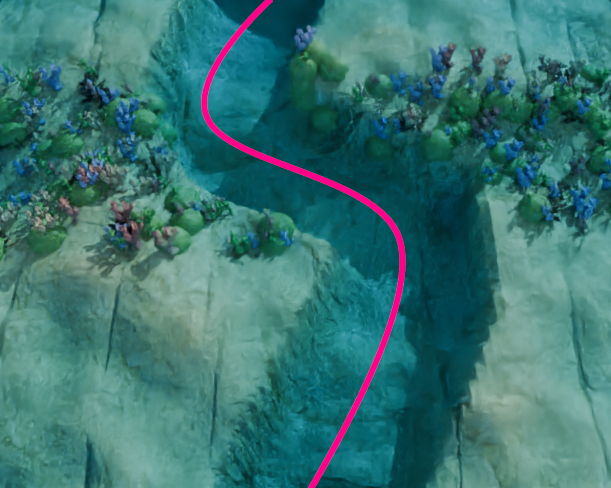
\includegraphics[width = 0.3 \linewidth]{Figures/Interactions/InteractionEdition1.png}
    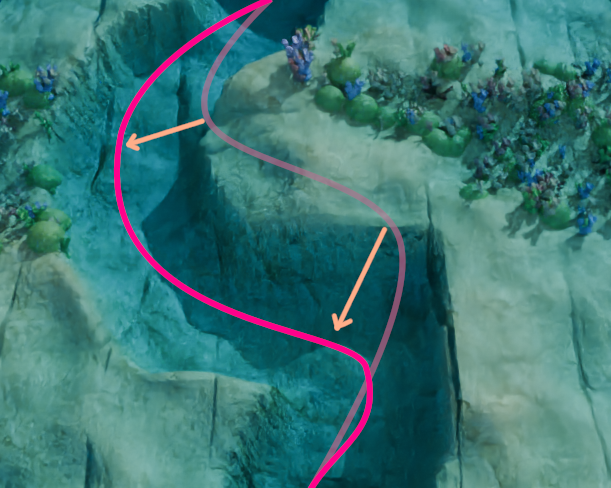
\includegraphics[width = 0.3 \linewidth]{Figures/Interactions/InteractionEdition2.png}
    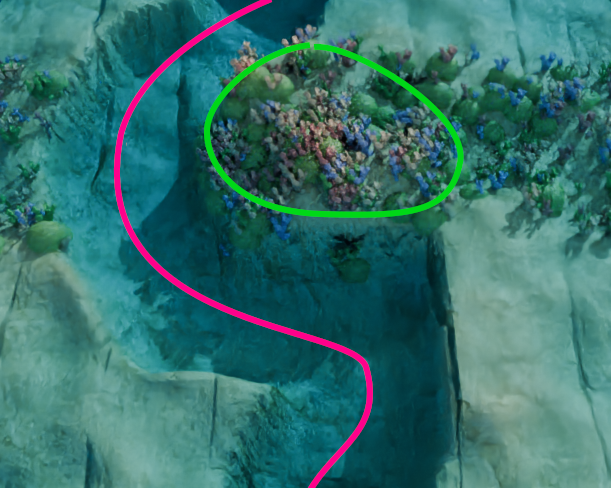
\includegraphics[width = 0.3 \linewidth]{Figures/Interactions/InteractionEdition3.png}
    \caption{Starting from a coral colony developed around a canyon (\textit{left}), the user edits the shape of the canyon, resulting in a different configuration of the scene, killing the corals that ends too deep in the water (\textit{center}) and the development and growth of new corals at the previous location of the canyon (\textit{right}). }
    \label{fig:semantic-representation_user-interaction}
\end{figure}

As long as a non-zero \gloss{FitnessFunc} is defined in the terrain, new \glosses{EnvObj} can be forced by the user at any point of the simulation. 

% \subsection{Guiding the simulation}
Control over the region of the terrain that should be updated can be given by adjusting all \glosses{FitnessFunc} through a scalar field $\influence: \R^2 \to \R $ such that the \gloss{FitnessFunc} $\fittingFuncObj(\p)$ of any new \gloss{EnvObj} is evaluated as $\fittingFuncObj^*(\p) = \influence{\p} \fittingFuncObj(\p)$. This is especially useful in the planning of robotic simulations as we can first generate the overall shape of our terrain and secondly focus the generation process around the areas that may be visited by the robot, avoiding useless simulations and computer power. 
Figure~\ref{fig:semantic-representation_coral-colonization-scene} shows an example of colonization of the coral polyps that we limited manually into an annulus.
% Figure~\ref{fig:semantic-representation_focus-area-example} shows an example of colonization of the coral polyps that we limited manually.

% \begin{figure}
%     % \centering
%     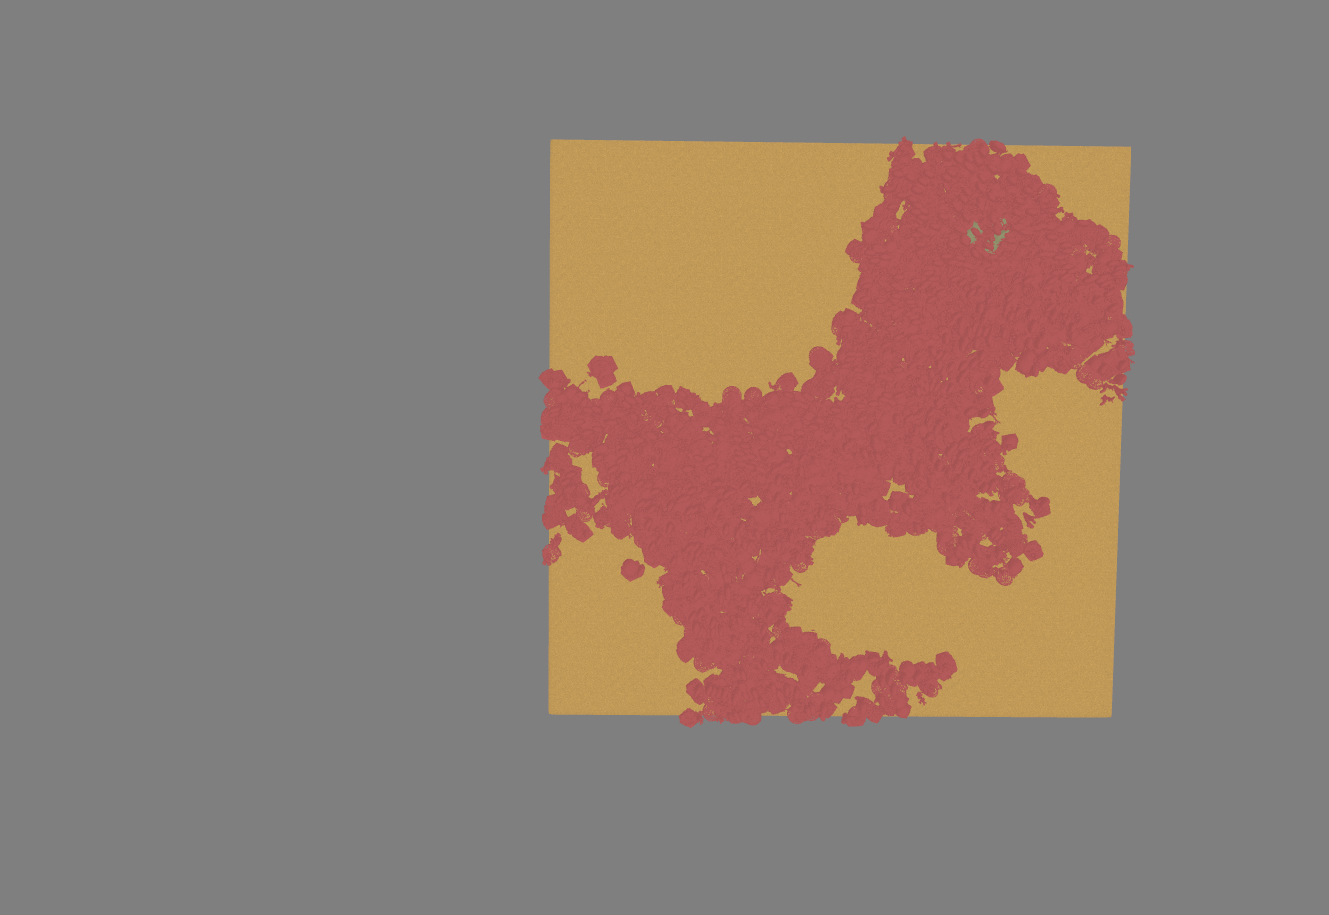
\includegraphics{Figures/UserControl/guidedGeneration1.png}
%     \caption{Controlling the generation area can produce a user-defined focused shape.}
%     \label{fig:semantic-representation_focus-area-example}
% \end{figure}

% - Changing the water currents

Our water current simulation is modeled as a simple vector field. As such, the user is able to interact with it at any moment of the simulation, allowing for the death of sensible \glosses{EnvObj} while it will guide the simulation into a new landscape. By modifying the water currents, the user also modifies the transport rate of \glosses{EnvMat} at this position. The modification of currents is given as a stroke, a parametric curve $\curve$ for which we evaluate $\Delta \Wuser(\p)$ just as for curved environment objects (Section~\ref{sec:semantic-representation_water-currents}).

\subsection{Indirect interaction of \glosses{EnvObj}}
\label{sec:semantic-representation_events}
A configuration file can define in advance the different \glosses{GeoEvent} that should be triggered during the simulation. This can be useful to generate landscapes that are close to some existing locations. 
Multiple \glosses{GeoEvent} can be triggered either as sudden or continuous environmental changes. These changes play a huge role in the morphology of landscapes.
We define \glosses{GeoEvent} with a starting point and an ending point, such that at any time of the simulation we can compute the progress of the \gloss{GeoEvent} as $\tEvent \in [0, 1]$.

Water level changes are important \glosses{GeoEvent} that shape the underwater landscapes. As previously submerged \glosses{EnvObj} get elevated above water level, flora and fauna terrain features dry and die. Deprived from the living part of the features, everything is more affected by terrestrial erosion. By updating the value of the depth $\depth$ evaluated in the \glosses{FitnessFunc}, any \gloss{EnvObj} that is sensible to the depth will be impacted automatically, that may be causing death (Figure~\ref{fig:semantic-representation_water-event}). The modification of the water level is defined as 
\begin{align*}
    \depth(\p) = \depth_0(\p) + \sum_{e \in \events} \Delta \depth_e \tEvent
\end{align*}
with $\Delta \depth_e$ the amount of water rising or lowering during an \gloss{GeoEvent}. We assumed a linear evolution of the water level during an \gloss{GeoEvent}. This allows to evaluate the depth at any point in space and in time.

\begin{figure}
    % \centering
    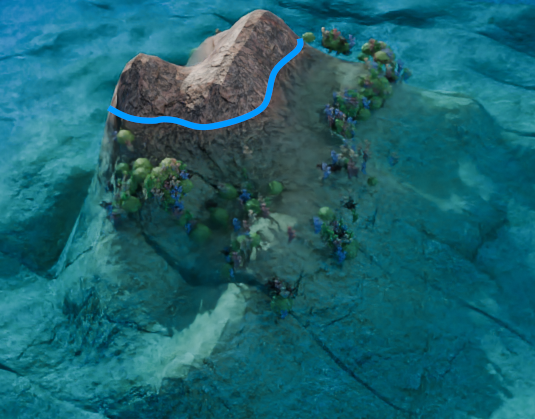
\includegraphics[width = 0.45 \linewidth]{Figures/Interactions/InteractionWater1.png}
    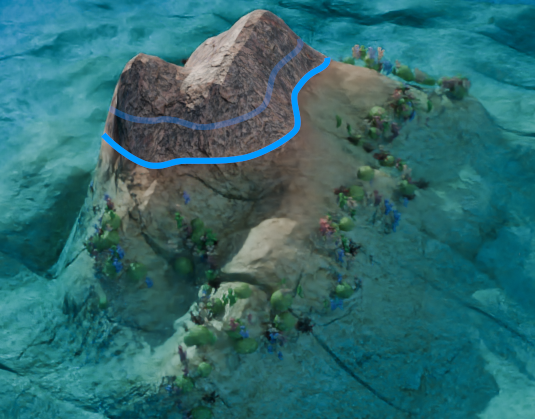
\includegraphics[width = 0.45 \linewidth]{Figures/Interactions/InteractionWater3.png}
    \caption{Lowering the water level by a few meters caused most of the coral objects to satisfy $\fittingFuncObj \leq 0$, causing their death. Since the water level (blue) decrease slowly, new coral objects spawn progressively at a lower altitude.}
    \label{fig:semantic-representation_water-event}
\end{figure}

Subsidence and uplift are the main \glosses{GeoEvent} that create or destroy islands in the long term. These \glosses{GeoEvent} are simulated as a simple factor on the height field of the generated terrain (Figure~\ref{fig:semantic-representation_subsidence-event}). Subsidence is not always uniform in the terrain. As such, the user can provide a position $\q$ at which the subsidence is the strongest, the amount of subsidence applied $\Delta \height_e$ and a standard deviation $\std$ for which we can then compute at any point in space and time of the simulation the height of the terrain
\begin{align*}
    \height(\p) = \height_0(\p) \cdot \sum_{e \in \events}{\frac{G(\norm{\p - \q})}{G(0)}} \Delta \height_e \tEvent 
\end{align*}
with $G(x)$ the Gaussian function
\begin{align*}
    G(x) = {\frac {1}{\std {\sqrt {2\pi }}}} \exp \left(-\frac {x^{2}}{2 \std ^{2}}\right)
\end{align*}

\begin{figure}
    % \centering
    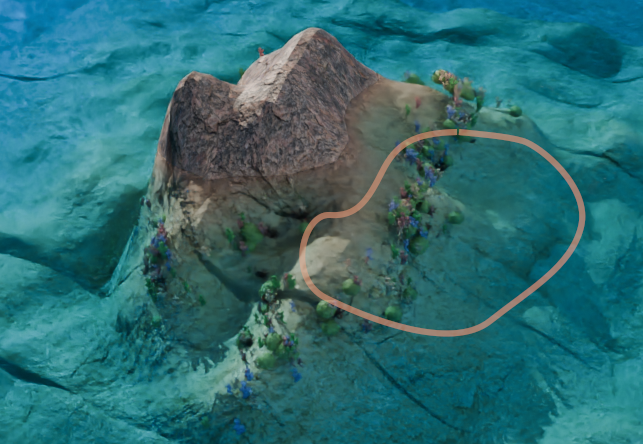
\includegraphics[width = 0.45 \linewidth]{Figures/Interactions/InteractionSubsidence1.png}
    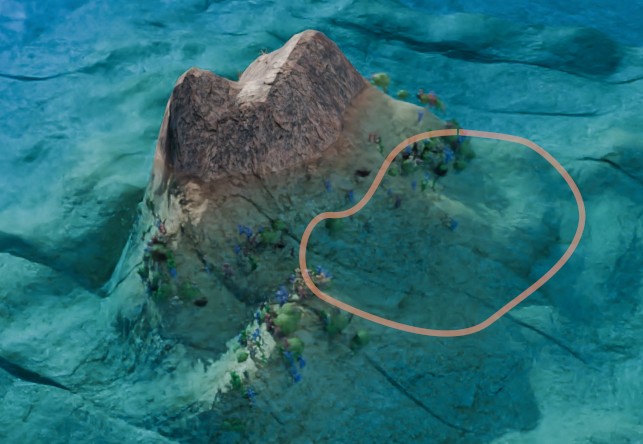
\includegraphics[width = 0.45 \linewidth]{Figures/Interactions/InteractionSubsidence2.png}
    \caption{Simulating subsidence on a part of the terrain (brown area) cause the depth value to change locally, resulting in the death of coral objects that find themselves too deep to survive. Here two subsidence \glosses{GeoEvent} are triggered in parallel. }
    \label{fig:semantic-representation_subsidence-event}
\end{figure}

Storms are factors of the geomorphology of coral reefs \cite{VilaConcejo2016, Oron2023} and coasts \cite{Dominguez2005, Cowart2010}. Due to the extreme wind and wave velocities coasts are highly eroded in a short time period and the more fragile corals near the water surface are broken, possibly causing breaches in the reefs and spreading polyps in the currents direction. While there are many factors at play to understand the apparition of storms and the hydrodynamics affecting it, we simplified the model of storms to the user as a single epicenter $\q$ with a wind velocity $\windVelocity$ and a standard deviation $\std$ representing the spread around the epicenter (Figure~\ref{fig:semantic-representation_storm-event}). The computation of water currents are then computed as 
\begin{align*}
    \Wuser(\p) = \Wuser^*(\p) + \sum_{e \in \events | \tEvent \in [0, 1]} {\windVelocity \frac{G(\norm{\p - \q}}{G(0)}}
\end{align*}
In this case, we did not include the linear factor $\tEvent$ as storms are usually conserving a constant force for the time of the few weeks or months of their occurrence. 

\begin{figure}
    % \centering
    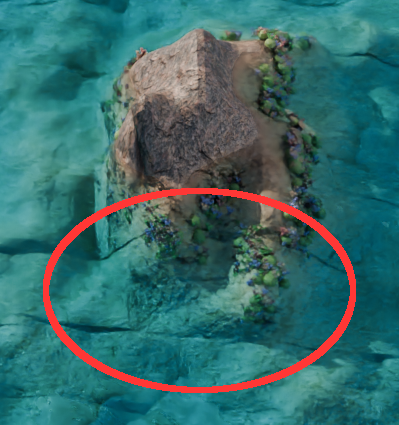
\includegraphics[width = 0.45 \linewidth]{Figures/Interactions/interactionStorm1.png}
    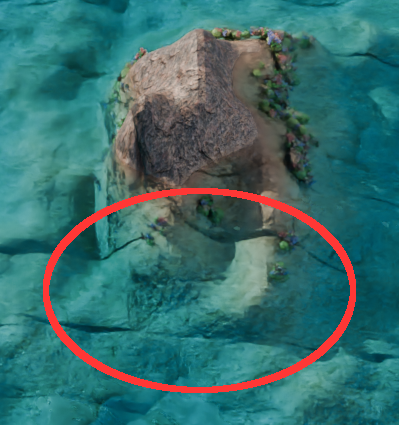
\includegraphics[width = 0.45 \linewidth]{Figures/Interactions/interactionStorm2.png}
    \caption{The result of a storm localized on one side of the island (red area) modifies the result of the evaluation of \glosses{EnvObj} around its epicenter for a short period of time. Most of the coral objects died from the \gloss{GeoEvent}, except few \glosses{EnvObj} less sensible to water currents strength. }
    \label{fig:semantic-representation_storm-event}
\end{figure}

% Just as for the rise and lowering of water level, the heat is modeled as a simple value of the environment. For shallow areas (<100m) we assume a linear relation between depth and temperature, and a constant value for the terrestrial environment. As such, we can model a heat wave by a change of the \glosses{EnvVal}. \Glosses{EnvObj} who are sensible to temperature may die instantly. The modification of the temperature is defined as 
% \begin{align*}
%     \temperature(\p) = T_0(\p) + \sum_{e \in \events} \Delta \temperature_e \tEvent + c \depth(\p)
% \end{align*}
with $\Delta \temperature_e$ the change of heat during an \gloss{GeoEvent}, $\temperature_0$ the temperature at the water surface, and $c$ a very small factor.

The framework can easily be extended as the \gloss{GeoEvent} system stays similar for all \glosses{GeoEvent}. Including higher level simulations in the \gloss{GeoEvent} system can be added, such as the simulation of tectonic activity, the use of fluid dynamics for tsunami \glosses{GeoEvent}, the integration of human activity, ...

\section{Results}
\label{sec:semantic-representation_results}
Our method provides a way to generate scenes at different scales. We demonstrate this capacity with the generation of a large scene of an island (Figure~\ref{fig:semantic-representation_teaser}) after what we focused the generation process in a canyon (Figure~\ref{fig:semantic-representation_canyon-scene}), then a small-scale visualization of coral colonies (Figure~\ref{fig:semantic-representation_coral-colonization-scene}).
In the examples, we rendered the \glosses{EnvObj} as a implicit tree or as individual meshes. The island, lagoons, reefs, canyons and sand ripples as implicit surfaces

% \subsection{Mid-scale}
% \label{sec:semantic-representation_mid-scale}
A canyon scene can be generated using our method. The water flow is affected by the curve of the canyon such that the currents are oriented in the direction of the curve's tangent.In this example, we force the position of arches to be inside the canyon. The arches deposits a material "rock deposit", which is the main element of the \gloss{FitnessFunc} of the Rock object. The "rock deposit" is slightly affected by water currents, but its mass make it highly affected by gravity. As such, rocks will spawn underneath arches. In reality, an arch is often created as part of a large coral boulder that sees the calcareous bottom part detached by the water currents, often resulting in an arch surrounded by big rocks and smaller rocks from the erosion of the first rocks.
As such, we define an \gloss{EnvObj} "Arch" with a \gloss{FitnessFunc} $\fittingFunc_{arch}(\p) = 5 - d(canyon - \p) * \norm{\Water(\p)}$, an \gloss{EnvObj} "Rock" using $\fittingFunc_{rock}(\p) = \material_{rock\_deposit}(\p)$ and Pebble using $\fittingFunc_{pebble}(\p) = \material_{smaller\_rock\_deposit}(\p)$. Finally, sand ripples are simply described as curves appearing where there is a lot of sand available: $\fittingFunc_{ripple}(\p) = \material_{sand}(\p)$.
Following these simple rules, Figure~\ref{fig:semantic-representation_canyon-scene} shows the emergence of details in the scene. 

% \subsection{Small-scale}
% \label{sec:semantic-representation_small-scale}
In this example we defined three different types of corals, coralA, coralB and coralC, to illustrate the possibility to model behaviours from the choice of \glosses{FitnessFunc}. Each of the coral types deposits a material "coral polyp" and "coral polyp A" ("coral polyp B" and "coral polyp C" respectively). By considering a \gloss{FitnessFunc} that minimize the ratio $\frac{\text{coral polyp}}{\text{coral polyp A}}$, we can see an emergent behavior of the three types of coral fighting for the space colonization.
Figure~\ref{fig:semantic-representation_coral-colonization-scene} shows the result of this simulation at three different interations. At the border between two colonies, none of the colonies make progression due to the amount of coral polyp specific from the other colony.

\begin{figure*}
    % \centering
    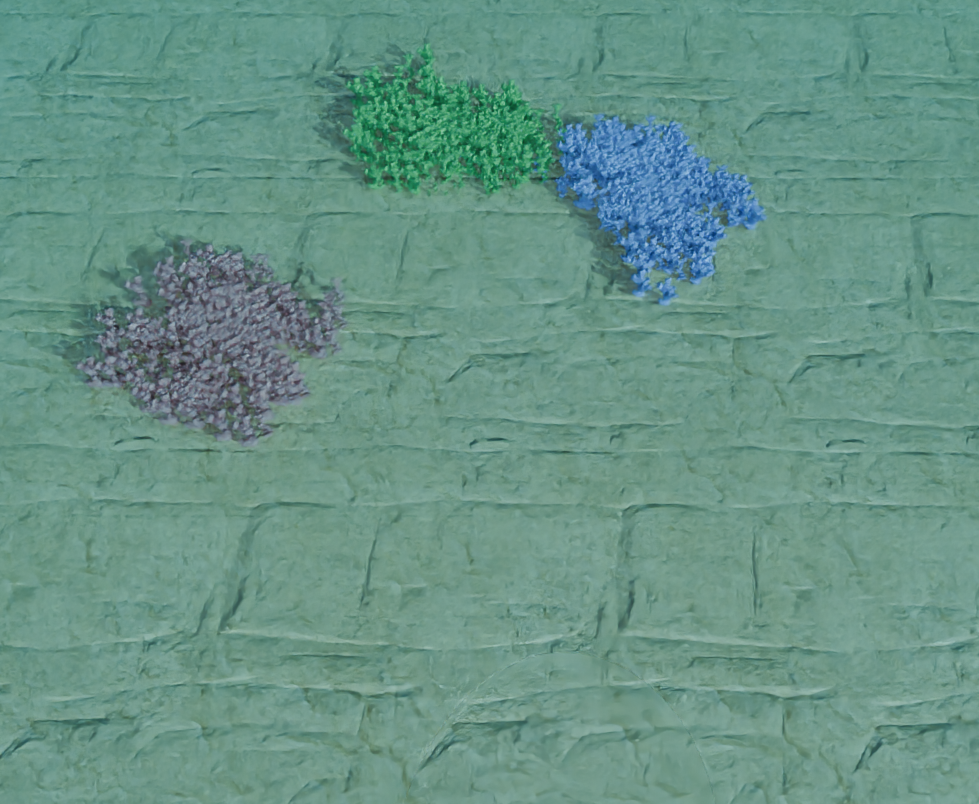
\includegraphics[width=0.24 \linewidth]{Figures/Colonization/col0.png}
    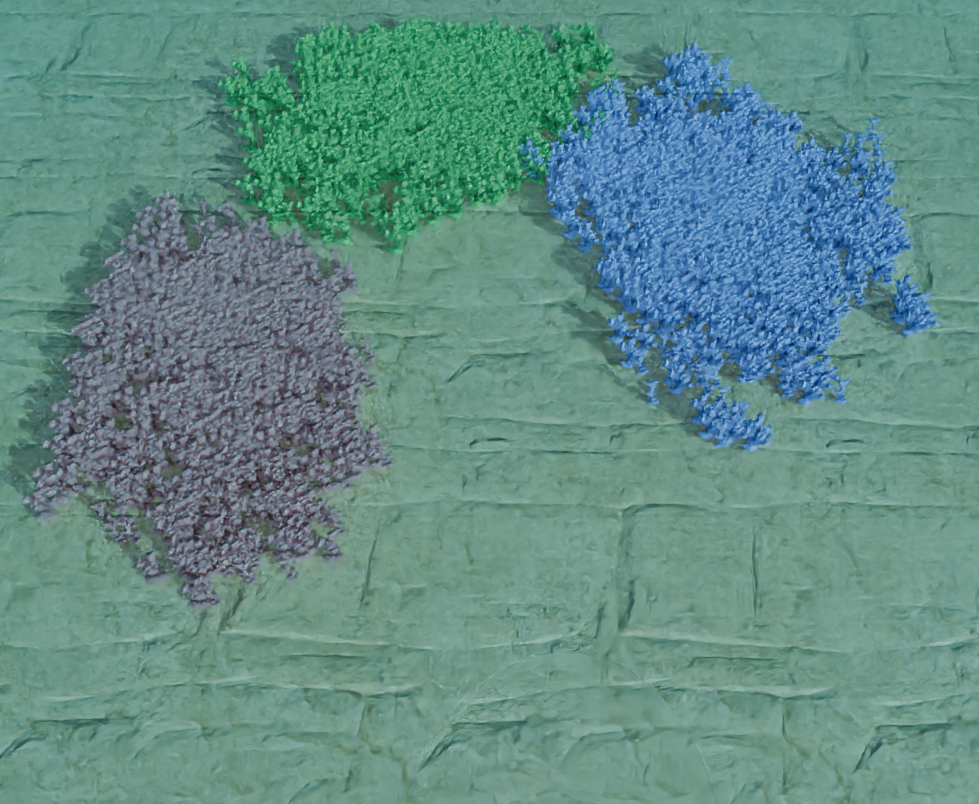
\includegraphics[width=0.24 \linewidth]{Figures/Colonization/col1.png}
    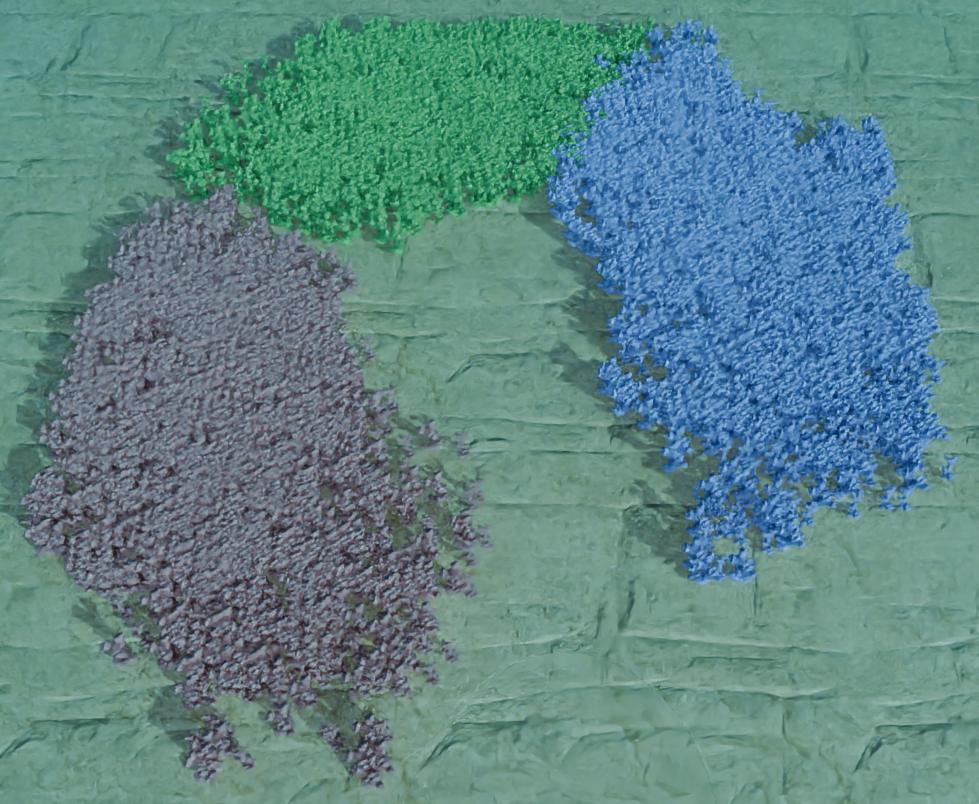
\includegraphics[width=0.24 \linewidth]{Figures/Colonization/col2.png}
    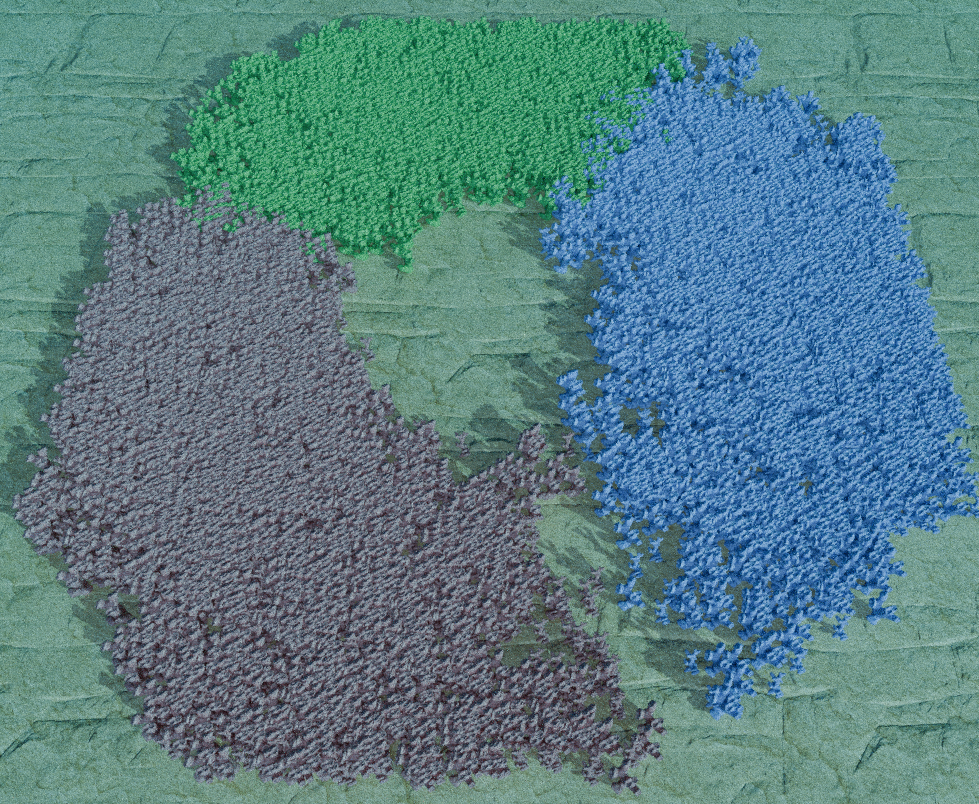
\includegraphics[width=0.24 \linewidth]{Figures/Colonization/col3.png}
    \caption{Three colonies of coral (red, blue, green) restricted to an annulus the middle section of the terrain fighting for the space.}
    \label{fig:semantic-representation_coral-colonization-scene}
\end{figure*}

\begin{figure*}
    % \centering
    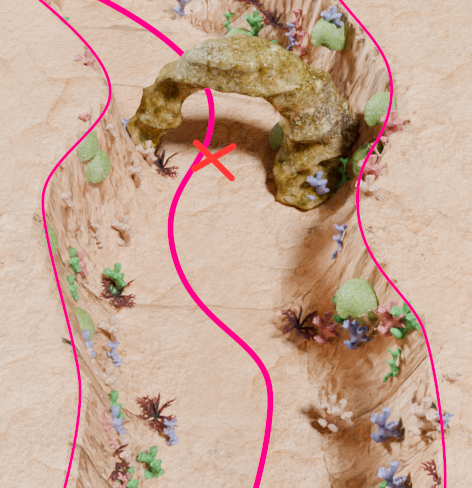
\includegraphics[width = 0.24 \linewidth]{Figures/Canyon/Canyon2.png}
    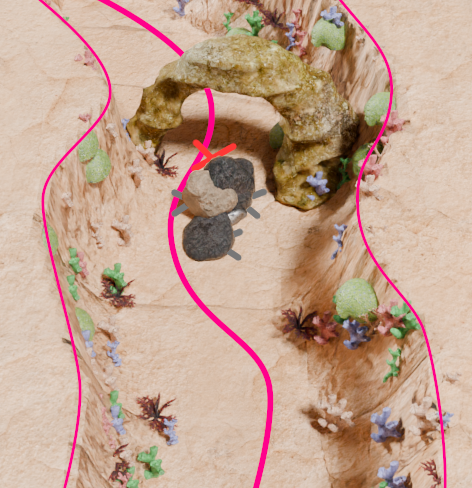
\includegraphics[width = 0.24 \linewidth]{Figures/Canyon/Canyon3.png}
    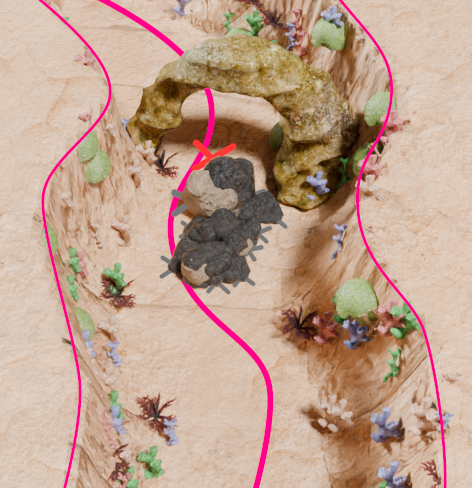
\includegraphics[width = 0.24 \linewidth]{Figures/Canyon/Canyon4.png}
    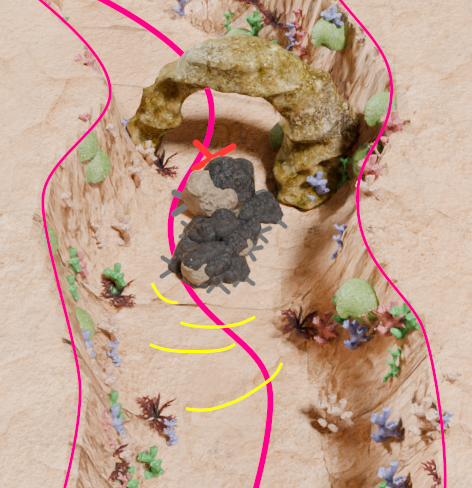
\includegraphics[width = 0.24 \linewidth]{Figures/Canyon/Canyon5.png}
    \caption{Evolution of a canyon scene at different iterations of the simulation. The apparition of an arch causes the spawning of rocks, pebbles, and finally some deposition of sand at the bottom of the canyon, spawning ripples. }
    \label{fig:semantic-representation_canyon-scene}
\end{figure*}


The proposed method aims to generate plausible landscapes using simplified versions of the evolution of an ecosystem and of the 3D representation. The biological realism of the result is highly correlated to the amount of simplification and assumptions, while the visual realism is completely dependent to the geometric functions used for the 3D modeling of the \glosses{EnvObj}. While proposing a flexible method that propose a generic approach for terrain generation, a close collaboration with fields experts and with graphists is needed to achieve optimal results.

Most simulation algorithm's quality depends on the size of the time step used, but with the introduction of a decay rate in the \glosses{EnvMat} properties, we limit the influence of time steps by considering that steady-state are reachable. The material deposition and absorption on punctual \glosses{EnvObj} can be seen as a Dirac function $\dirac$ centered at their position resulting in the advantage that material displacement function can use the definition of the diffusion equation instead of the advection-diffusion-reaction equation. This equation allowing us to evaluate the state of the material $\material$ without intermediate steps, but this is not applicable with curve- and region-based \glosses{EnvObj}. 

\section{Conclusion}
\label{sec:semantic-representation_conclusion}
We have proposed a method to generate terrains procedurally using sparse representations. This representation, the \glosses{EnvObj}, enables to introduce expert knowledge by the mean of the \glosses{FitnessFunc} that rule the \glosses{EnvObj} life cycle, but also to integrate the user in the loop during the generation process. We reduced the terrain resolution limitations by defining the environment objects as parametric features. Thanks to the sparse representation based on single points, curves and regions, we allow for direct manipulation of the \glosses{EnvObj} of the scene by the user which, thanks to the environment steady state consideration, also enables to include these interactions in the automatic simulation process.
Integrating environmental properties in the \gloss{FitnessFunc} of \glosses{EnvObj} allows the user to guide the generation through \glosses{GeoEvent}. Our method enables each \gloss{EnvObj} of the scene to influence the environment locally, reducing the need of computations while also retrieving \glosses{EnvVal} locally, which result in a parallelizable life-like simulation process. The genericity of the environment properties definitions should be sufficient for plausible generation of other landscape types as long as expert knowledge can be translated to \gloss{EnvObj}'s formalism.


We limited our work to the use of 2D scalar fields as they are more easily differentiable, interpretable and lighter than volumetric representations. However, future works include using 3D representations of the terrain and the environment to generate 3D terrains, including cavities, sub-terrestrial areas and the interior of coral structures. 
% The different possibilities to explore for this would be: the use of 3D particles to represent the state of the \glosses{EnvMat} in the environment, or voxel grids or flatten representation of the terrain's surface (but would not allow a different morphological shape than the height field...).

\begin{figure*}
    % \centering
    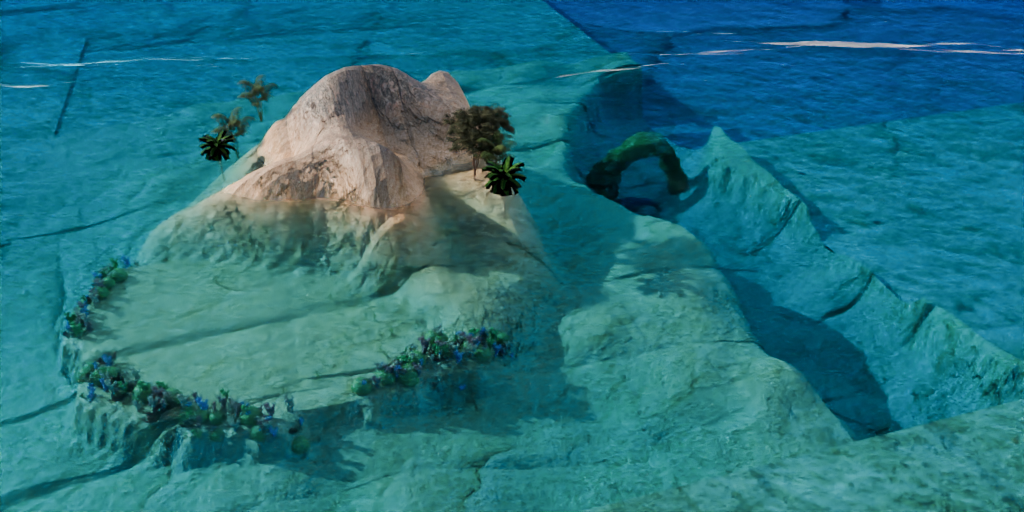
\includegraphics{Figures/CoralIsland/multiScene1 v2 final 1.png}
    \caption{A simple coral island is generated using an island, a lagoon, reefs coral polyps, beaches, trees and algae \glosses{EnvObj}. Trees appear on beaches and algae grow in the lagoon's sand. }
    \label{fig:semantic-representation_coral-island-scene}
\end{figure*}














% \section{Method}
% \label{sec:semantic-representation_method}
% The overall pipeline of the method is based on simple incremental generation like most rule-based systems. In this type of system, the final state is defined either by reaching equilibrium, or by verifying specific conditions, such as a maximum number of iterations. 
% We define our pipeline in three phases (Figure~\ref{fig:semantic-representation_pipeline}): the initialization phase that describe the generation and simulation rules, the iterative phase generating populating the terrain with our \glosses{EnvObj} and finally the output.


% \subsection{Pipeline overview}





















% \section{Expert knowledge integration}
% \label{sec:semantic-representation_biology}
%   The definition of the \glosses{FitnessFunc} of the \glosses{EnvObj} are inspired by the biological and geological factors that rule the evolution of underwater landscapes. The main factors are depth, light, water currents and biodiversity. External \glosses{GeoEvent} have direct and indirect repercussions on the biodiversity of underwater environments. Coral islands are complex bio systems in which fauna, flora and geology are mixed together. 

% \subsection{\Glosses{EnvObj} description}
% \label{sec:semantic-representation_represented-objects}
% We have represented with \glosses{EnvObj} some geologic features, animal features and flora features. The low island is most often raised in a circular shape as the process mainly appear around a hot spot under the ground. The evolution of an island into a coral island requires that the environmental conditions are sufficient for coral development: corals will grow slightly below the water surface as waves will break its growth and at a shallow depth (around 3m to 30m deep) in order for light to reach it. As coral grow and die, the skeleton is transformed into porous limestone, providing shelter to surrounding animals and reducing the impact of water erosion on the island. Corals drop polyps that are transported by the water flow and when they stick to a hard surface, as a rock or the reef itself, the coral may grow and colonize the area. As subsidence cause the island to lower, the living part of the coral reef keep growing toward light, which lead to a reef that is constantly close to the water level without reaching it due to wave erosion. The survival of reefs depends on the equilibrium between coral growth and and erosion. Eroded parts of the reef falling in the sheltered part of the reef accumulates, ending up by forming a lagoon. An island formed by a hot spot will inevitably subside in time, until it is completely flatten. As the coral reefs keep growing, only the lagoon remain, resulting in an atoll. \\
% In this work we we integrate the biological and geological knowledge in the \glosses{FitnessFunc} of the \glosses{EnvObj} we want to generate. We represent the islands as regions that can be appearing with a uniform distribution. From the formulation of the region description \eqref{eq:internal-energy-equation}, we mostly create circular islands. The coral features, \glosses{EnvObj} described as a single point, have a \gloss{FitnessFunc} that take into account the depth of the ground, the amount of sand, fresh water and polyps in their environment, as well as the strength of water currents. Each coral species have different living conditions, but we reduced our work to soft coral which are sensible to water strength and stony corals that are more resistant to erosion. Reefs are formed as coral's skeleton are transformed into calcareous stone, describing then as an \gloss{EnvObj} representing multiple others. 

% \subsection{Simplifications}
% \label{sec:semantic-representation_simplifications}
% The environmental factors simulated are greatly simplified as the real processes are in a very small time scale, that computer simulation are not able to simulate in interactive time. The use of \glosses{EnvObj} aim to represent a plausible results, while avoiding modeling the smaller scale \glosses{GeoEvent}. Examples of simplifications are the geometry and material of each \gloss{EnvObj}, which have an influence on the water currents through friction, the water currents represented as stationary flows, while the water flow dynamics are a complex system that may change completely at two different times of the day, the animal influence on the reefs that they transform by the ingestion and deposition of sediments, ...

%
%- What is semantic representation? \\
%** Linguistic definition + Image definition + Our definition \\
%- Why use semantic representation? \\
%** Sharing knowledge with biologists, geologists, etc. \\
%** Data from travel journals, labeled maps, ... \\
%- Advantages and disadvantages of semantic representation \\
%** Advantages: \\
%*** Interpretation \\
%*** User control \\
%*** 3D representation abstraction \\
%** Disadvantages: \\
%*** Need for expert knowledge (+ interdisciplinary communication issues) \\
%*** Necessary simplifications in physics / natural phenomena \\
%- 3D representation of semantic terrains \\
%** Possible combinations of methods (implicit functions + meshes)
%
%\section{Sparse Terrain Representation}
%- Landscape contains structures of very varying sizes: \\
%** Mountains covering several km² but rivers a few meters wide, for example \\
%- Proposal for sparse terrain representation \\
%** Definition of terrain elements as simple objects: environmental objects \\
%** Implicit geometry, offering 2D or 3D display \\
%** "Easy" LOD possibility \\
%- Iterative method for generating sparse terrain \\
%** Reduce computation time from $O(n^2)$ to $O(n)$ by using the environment as a proxy \\
%** Method based on material deposition \\
%** Iterative stochastic process
%
%\section{Environmental Objects}
%- Symbolism of the environmental object \\
%- Reference to "Environmental Objects" \\
%- Comparison to biotopes
%
%\subsubsection{Definition}
%- Skeleton \\
%- Parametric shape \\
%- Living conditions
%
%\subsubsection{Implementation}
%- Instantiation of objects \\
%** Definition of the skeleton \\
%*** Points, curves, regions \\
%*** Use of Snake \\
%** Definition of geometry \\
%- Modifications to the environment \\
%- ...
%
%% \chapter{Snake - Active Contour Model}

We want to symbolize a dead coral area as a \gloss{EnvObj} "reef." To do this, the coral objects continuously deposit a quantity of "dead coral" material. This material, stored in a discrete scalar field, contains high intensities where a reef should supposedly exist. 
We need to draw a curve to represent this new object. The constraints of this curve are that it must pass through the points of highest intensity while maintaining a given length.

The Snake algorithm, or Active Contour Model, approaches this application. The algorithm proposes to give an energy to the curve, which then tries to minimize it through gradient descent.

The energy, in the initial paper, is defined by
\begin{align}
    \Esnake^{*} = \int \limits _{0}^{1} { \Esnake(\mathbf {v} (s))\,ds } = \int \limits _{0}^{1} { \Einternal (\mathbf {v} (s)) + \Eexternal (\mathbf {v} (s)) } \,ds
\end{align}

The internal energy represents the properties of the curve while the external energy represents properties of the field it lies in. In the original paper they are described as: 
\begin{align}
    \Einternal &= \alpha \Econt + \beta \Ecurv \\
    \Eexternal &= \gamma \Eimage
\end{align}

The continuity cost $\Econt$, originally defined as the minimization of the spacing between the points $\left\|{\frac {d{\bar {v}}}{ds}}(s)\right\| ^{2}$, does not make much sense in the discrete form of the algorithm. In its discrete form, we seek to maintain a regular interval between the points by applying $\Econt = \left(\tilde{d} - \left\|p_i - p_{i-1} \right\| \right)^2$ with $\tilde{d}$ being the average distance between each point.

The curvature cost $\Ecurv$ seeks to minimize the oscillations of the curve and can thus be defined as the squared second derivative $\left\|{\frac {d^{2}{\bar {v}}}{ds^{2}}}(s)\right\| ^{2}$.

The discrete form $\Ecurv^{*} = \left\| p_{i-1} - 2 p_i + p_{i+1} \right\| ^2$ is not necessary with splines, due to their closed form.

The image cost $\Eimage$ tries to attract the points of the curve to a local maximum of the image gradient. It is defined as $\Eimage = - \left\| \nabla I \right\| $.

We want to see our curve maintain a given length $L$. We then modify the formulation of the continuity cost to become $\Econt = \left(\tilde{l} - \left\|p_i - p_{p-1} \right\| \right)^2$ with $l = \frac{L}{n - 1}$, knowing $n$ is the number of vertices of the curve. Additionally, we want a curve that follows points of high intensity rather than the gradient, which leads to modifying the image cost $\Eimage = -I$.

The calculation of the gradient $\nabla \Esnake$ remains trivial in parts:
\begin{align}
    \frac{\partial \Eimage}{\partial p_i} &= - \nabla I(p_i) \\
    \frac{\partial \Ecurv^{*}}{\partial p_i} &= -\frac{2 \left( p_{i-1} - 2 p_i + p_{i+1} \right) }{ \left\| p_{i-1} - 2 p_i + p_{i+1} \right\| } \\
    \frac{\partial \Econt^{*}}{\partial p_i} &= 2 \left(l - \left\|p_i - p_{i-1} \right\| \right) \cdot \frac{p_i - p_{i-1}}{ \left\| p_i - p_{i-1} \right\| }
\end{align}

We then have
\begin{align}
    \Esnake &= \alpha \left(l - \left\|p_i - p_{i-1} \right\| \right)^2 + \beta \left\| p_{i-1} - 2 p_i + p_{i+1} \right\| ^2 - \gamma I \\
    \nabla \Esnake &= 2 \alpha \left(l - \left\|p_i - p_{i-1} \right\| \right) \cdot \frac{p_i - p_{i-1}}{ \left\| p_i - p_{i-1} \right\| } - \beta \frac{2 \left( p_{i-1} - 2 p_i + p_{i+1} \right) }{ \left\| p_{i-1} - 2 p_i + p_{i+1} \right\| } - \gamma \nabla I(p_i)
\end{align}

It should be noted that the calculation of $\Econt^{*}$ uses the distance $\left\|p_i - p_{i - 1} \right\|$. For $i = 0$, the distance $\left\| p_i - p_{i + 1} \right\|$ is used.

If all the points of the curve are at a distance greater than $l$, the optimization will push each of these points to get closer to its predecessor. Point $p_0$, itself, will move very little, so the entire curve aligns towards point $p_0$. By using the distance to the successor $\left\| p_i - p_{i+1} \right\|$, the curve moves towards point $p_N$.
It is then possible to converge towards the median point by alternating the use of the distance with the predecessor and with the successor, at the cost of slower convergence.

The active contour model algorithm is highly sensitive to the initial curve placement. In cases where a portion of the curve is in an area with a very low gradient on $\Eimage$, the vertices of the curve will simply optimize $\Einternal$, resulting in a straight segment in a low-intensity area, while the rest of the curve optimizes correctly.

To mitigate this problem, we propose adapting the Snake algorithm into Caterpillar: throughout the gradient descent, the target length $L$ is artificially reduced and then increased. In this way, a portion of the curve blocked in a region without possible optimization on external energy will be attracted by the optimized curve until it falls on a strong gradient. The dead portion can take the place of optimized vertices. By returning the target length $L$ to its initial value, the optimization continues with fewer vertices in the dead zone. Repeating this process gradually brings all points into an optimizable area. However, a too-rapid change in the target length can prevent the vertices from optimizing $\Eexternal$ by amplifying $\Einternal$ too much. Additionally, this algorithm can lead to numerical errors and slower convergence.

%
%\subsection{Communication between Objects}
%- Comparisons with reality \\
%** No direct communication between elements \\
%- ...
%
%\subsubsection{Interactions through the Environment}
%- Modifications to the environment \\
%** Absorption \\
%** Deposition \\
%** Modification of currents \\
%- Impact of the environment on objects \\
%- ...
%
%\subsubsection{Lifecycle of Environmental Objects}
%- ...
%
%\section{Results}
%- ...


%\subsection{Implemented Tools}
%- Cost function parser \\
%- ...

%\section{Other Attempts}
%\subsection{Direct Interactions}
%\subsubsection{Graph Generation}
%\subsubsection{Delaunay Triangulation}


%
%\section{Continuous Erosion}
%[POSSIBLY TO BE MOVED TO EROSION] \\
%- ...
%
%\subsection{Problem Description}
%- Erosion process is a dynamic system \\
%- Very large number of variables \\
%- Impossible to simulate at different time steps and/or different scales/resolutions
%
%\subsection{Proposed Solutions}
%- ...
%
%\subsubsection{Lifecycle of Environmental Objects}
%- ...
%
%\subsubsection{Use of Deep Learning}
%- ...




%\chapter{Influence sur la génération}
\label{chap:influence-on-env-objects}
\minitoc


\section{Introduction}
\label{sec:influence-on-env-objects_introduction}
This document aims to formalize a terrain generation method developed during my thesis.

The main issue this method seeks to address is the difficulty for a user to describe the environments they want to generate. By proposing a hierarchical structure in the description of elements to define, the environments exhibit adaptive representation granularity, catering both to the user's needs and hardware capabilities.

The key element of the method is the "biotope," defined as "a habitat defined by relatively uniform physical and chemical characteristics." (Source: Wikipedia)

In this context, we define the characteristics of a geographical region as well as the sub-biomes included within it.

Although this method was conceived with the aim of generating underwater environments, many examples given in this document will use elements present in surface environments, purely for simplification purposes.

\section{Glossary}
\label{sec:influence-on-env-objects_glossary}
Initially, this document will present definitions of various terms used in the description of the method. By doing so, we hope to eliminate any ambiguity in the upcoming explanations. Definitions may appear in certain sections of this document if deemed too specific.

\textbf{Biotope}: The main element of the method used. The biotope (or, as I might often write, the biome) is a geographical region defined by topographic and geomorphological characteristics. The notion of biotope used does not distinguish between different scales (the biosphere and the ecosystem of a rock are represented uniformly), nor does it distinguish between living and mineral elements. The biotope is represented in two different ways in the terrain generation process: the model and the instance.

\textbf{Model (of biotope)}: The model (or biotope model, if the context requires) is a biological description of the geographical area. It remains an abstract, or literary, form of the biotope. It is defined by a list of characteristics related to topography (description of the relief, description of the shape of the region) and geology (type of soil, for example). One can also list the sub-biomes that compose it, specifying the quantity, proportion, chances of appearance, etc., of each sub-biome. This form is the user input into the system, but during the terrain generation process, the model's role is to create instances of itself to concretize the structure to be generated. In the document illustrations, if a model is represented in a graph, it will be symbolized by its name in quotation marks (e.g., "Forest," "Lagoon").

\textbf{Instance (of biotope)}: The instance is the concrete form of the model. Unlike the model, the instance takes place in space with fixed characteristics (unlike the probabilistic characteristics of the model). Through generation rules and living conditions defined by the user and the system, the biotope instance has a geometric shape and neighboring relationships with other instances. An instance, like its original model, consists of sub-biomes. The instance remains linked to its original model. To distinguish the instance from the model in the document illustrations, if represented in a graph, the instance will be symbolized by the model's name followed by a hash and an instance number (e.g., Forest \#1, Lagoon \#28).

\textbf{Generation Rule}: Generation rules represent a list of obligations or prohibitions, including living conditions and adjacency rules.

\textbf{Living Condition}: In our definition, a biotope can only exist under certain environmental conditions in a specific place. The conditions can be multiple and will be listed in a subsequent chapter of this document. Vegetative elements, for example, have strong constraints in terms of sunlight exposure, the "snow" biotope requires a low temperature condition, and some biotopes like sand cannot exist on steep terrain. Living conditions are therefore important properties to express in biotope models. These conditions can be expressed probabilistically.

\textbf{Adjacency Rules}: Adjacency rules define how biotope instances can be arranged. There are three types of rules to express adjacency between two biotopes: prohibition, possibility, and obligation. Two models linked by an adjacency prohibition cannot generate instances with a common border. Conversely, a model linked to another by an obligation constraint can only generate an instance if it shares a border with an instance of the linked model. The possibility constraint is the default, where the instance is indifferent to the presence or absence of a common border. It is conceivable that the notion of "possibility" could be associated with a probability in the future, allowing for example, a lake to often be adjacent to an urban area, but an urban area to rarely be near a desert. For now, adjacency rules are bilateral: a rule that applies from biotope A to biotope B also applies from B to A. In the rest of the document, adjacency rules will mainly be represented by graphs (undirected) with the nodes as the models to be generated, solid edges representing the possibility of adjacency, dotted edges symbolizing an adjacency obligation (rarely used), and the lack of an edge indicating an adjacency prohibition.

\textbf{Adjacency Graph}: The adjacency graph, although similar to the representation of adjacency rules, this time represents the concrete topological adjacency between the generated instances (not the models). The adjacency graph consists of nodes representing each instance generated by the models and the edges representing the existence of a common border. Edges can only be present if the two biotope instances see their model linked either by an obligation or possibility of adjacency constraint. By definition, this graph must be planar. In this document, adjacency graphs will therefore be represented by graphs where the nodes are biotope instances (following the instance graphic convention), and an edge represents a topological adjacency.

\textbf{Region (of biotope)}: The region is the space occupied in a geometric sense by a biotope instance once represented in space. Among the important properties, one can note that a region has a shape and an area.

\textbf{Boundaries}: The boundary is the geometric adjacency of two regions representing biotope instances.

\textbf{Adjacent Regions}: Two regions are adjacent if they share a common edge. In a successful generation, a region shares a common boundary with regions represented by instances linked to the current region instance in the adjacency graph. We can then distinguish three types of connections between instances: correctly adjacent instances are linked in the adjacency graph and are adjacent regions, over-adjacent instances are not linked in the adjacency graph and are adjacent regions, and under-adjacent instances are linked in the adjacency graph and are not adjacent regions. The latter two types are maladjacencies.

\textbf{Biotope Characteristics}: Biotopes possess characteristics common at all scales, whether they represent geological or biological elements. The characteristics are defined in the models in probabilistic forms. Instances inherit a unique and fixed value for each characteristic from the original model. The characteristics notably define the shape the generated region will take, the relief, etc.

\textbf{Sub-biotope}: Each biotope can include one or more sub-biomes. This is how an environment can be defined on the scale of a planet as well as on the scale of a rock. The biotope specifies the number of instances to generate for each sub-biome, or the proportion of the surface to cover. The parent biotope provides an approximate description of its environment, but with each sub-biome, the description is refined.

\textbf{Recursive Tree}: The proposed method has a strong recursive nature through its representation in biotopes and sub-biomes. The biotope construction tree is thus a recursive tree of biotopes composed at the root of a biotope to be generated and whose nodes (and leaves) represent sub-biomes. The parent-child relationship defines the inclusion of the child among the sub-biomes of the parent node. The tree describing a biotope can then be reused to describe a larger biotope, up to a planetary scale or larger.

\textbf{User Action}: The user plays an important role in the terrain generation process. By user action, we mean any action performed during the process. User actions are applied to biotope instances: adding, replacing, or deleting an instance, or modifying the characteristics and living conditions of an instance.

\textbf{Primitives}: Primitives are simple geometric representations that can be combined to represent more complex structures. Among these, we can notably find: the point, the curve, the sphere, and the 3D model.

\section{Environment description}
\label{sec:influence-on-env-objects_environment-description}
In this method, an environment is defined by a biotope model for which characteristics such as the general shape of its region, the biotope's relief, or the representative primitive of the biotope are specified, as well as living conditions such as altitude, temperature, and necessary luminosity for its survival. These characteristics are uniform across the entire biotope region; the only way to vary them is to add sub-biomes in the definition, which will take the form of sub-regions of the parent. Sub-biomes have the same types of characteristics and living conditions, which they can define in their own way, as well as their own sub-biomes.

Thus, the environment description is carried out recursively until the level of detail is sufficient for the modeler.

A biotope model can be the sub-biome of several different biotope models, offering the possibility to define complex environments quickly.

\subsection{Biotope characteristics}
The biotope model allows the user to describe the biotope's appearance to be generated. This description is probabilistic, and instances derived from the model each define a unique value for each characteristic respecting the probability law described by the model. The list of characteristics includes:
\begin{itemize}
	\item Region size: This represents the area of the surface (without considering relief) that the region occupies in space.
	\item Altitude (min and max): These two characteristics represent the altitudes the biotope can reach.
	\item Relief (frequency and amplitude): These characteristics describe the terrain's gradient. High relief amplitude symbolizes significant disturbances on the ground, unlike low amplitude, which
	
	indicates the ground is relatively flat.
	\item Primitive (type, dimension, position): The primitive determines the basic element represented by the biotope.
	\item Shape: The biotope region's shape in space.
\end{itemize}

To facilitate the user's work, default values are proposed for each biotope, respecting each type of primitive.

\subsection{Living conditions}
The living conditions of a biotope define the specific properties necessary for the biotope to survive. To be viable, the biotope must respect these conditions. These properties may relate to the following conditions:
\begin{itemize}
	\item Luminosity (min and max)
	\item Temperature (min and max)
	\item Soil type
	\item Exposure (direction, minimum and maximum angle)
\end{itemize}

Like characteristics, default living conditions are proposed to the user.

\subsection{Adjacency rules}
Three types of rules express adjacency between two biotopes: prohibition, possibility, and obligation. These rules define how biotope instances can be arranged spatially.

\begin{itemize}
	\item Prohibition: Two models linked by an adjacency prohibition cannot generate instances with a common border.
	\item Possibility: Instances can be adjacent, but it is not required.
	\item Obligation: Instances must share a common border.
\end{itemize}

\section{Generation process}
\label{sec:influence-on-env-objects_generation-process}
The terrain generation process involves creating instances from biotope models while respecting their characteristics, living conditions, and adjacency rules. This section details the steps of the process.

\subsection{Instance creation}
Each biotope model creates instances with fixed values for each characteristic derived from the probabilistic descriptions in the model. These instances are then positioned in space according to their characteristics and living conditions.

\subsection{Placement and adjustment}
Instances are placed in the environment, respecting their adjacency rules. If instances violate adjacency constraints, adjustments are made to either reposition instances or modify their characteristics within acceptable limits.

\subsection{User interaction}
Users can intervene in the generation process by adding, replacing, or deleting instances, as well as modifying instance characteristics and living conditions. These actions allow for fine-tuning the generated environment.

\subsection{Validation and refinement}
The final step involves validating the generated environment by checking for over- or under-adjacencies and making necessary refinements to ensure all instances adhere to their constraints and living conditions.

\section{Conclusion}
\label{sec:influence-on-env-objects_conclusion}
This method provides a structured approach to terrain generation by leveraging biotopes and their hierarchical organization. By defining biotopes probabilistically and respecting adjacency rules and living conditions, it is possible to generate diverse and realistic environments with varying levels of detail.

Future work may include refining probabilistic models for characteristics and adjacency rules, as well as exploring the use of probabilistic adjacency possibilities to further enhance the flexibility and realism of generated terrains.
%- ...
%
%\section{Biotope Generation}
%- ...
%
%\subsection{Definition}
%- ...
%
%\subsubsection{Recursion}
%- ...
%
%\subsubsection{Voronoi Diagram}
%- ...
%
%\subsubsection{Communication between Biotopes}
%- ...
